\documentclass[12pt,a4paper]{article}

\usepackage[margin=10pt,font=footnotesize,labelfont=bf]{caption}
\usepackage{epsf}
\usepackage{amsmath}
\usepackage{amssymb}
\usepackage{graphics, graphicx}
\usepackage{wrapfig}
\usepackage{caption}
\usepackage{subcaption}
\usepackage{latexsym}
\usepackage{hyperref}
\usepackage[latin1]{inputenc}
\usepackage[round,comma,authoryear]{natbib}
\usepackage{tabularx}
\usepackage[usenames,dvipsnames]{xcolor}
\usepackage{booktabs}
\usepackage{makeidx}
\usepackage{blindtext}
\usepackage{adjustbox}
\usepackage{varwidth}
\usepackage{color}
\usepackage{titlesec}
\usepackage{amsthm} % Theorem environment
\usepackage{mathabx}
\definecolor{CornFlowerBlue}{rgb}{0.392157,0.584314,0.929412}
\definecolor{LightGray}{gray}{0.8}

\newcommand{\sectionbreak}{\clearpage}
\newenvironment{defbox}[1]{%
	\vspace{0.3cm}
    \noindent
    \adjustbox{innerenv={varwidth}[c]{0.9\linewidth},margin=\fboxsep+.4cm \fboxsep+.35cm,bgcolor=LightGray,frame,center}\bgroup
    	\textbf{Definition: #1} \normalfont \newline
}{\egroup \vspace{0.3cm}}

\newenvironment{bbbox}[1]{%
	\vspace{0.3cm}
    \noindent
    \adjustbox{innerenv={varwidth}[c]{0.9\linewidth},margin=\fboxsep+.4cm \fboxsep+.35cm,bgcolor=LightGray,frame,center}\bgroup
    	\textbf{Blackboard: #1} \normalfont \newline \flushleft
}{\egroup \vspace{0.3cm}}

\newenvironment{exbox}[1]{%
	\vspace{0.3cm}    
    \noindent
    \adjustbox{innerenv={varwidth}[c]{0.9\linewidth},margin=\fboxsep+.4cm \fboxsep+.35cm,bgcolor=CornFlowerBlue,frame,center}\bgroup
    	\textbf{Example: #1} \normalfont \newline
}{\egroup \vspace{0.3cm}}

\newtheoremstyle{break}
  {\topsep}{\topsep}%
  {\itshape}{}%
  {\bfseries}{}%
  {\newline}{}%
\theoremstyle{break}
\newtheorem{proposition}{Proposition}[section]
\newtheorem{definition}{Definition}[section]
\newtheorem{theorem}{Theorem}[section]
\newtheorem{example}{Example}[section]

% Page setup
\textwidth 16cm
\textheight 22cm
\topmargin 0.0cm
\evensidemargin 0cm
\oddsidemargin 0cm
\parskip0.5explus0.1exminus0.1ex

% Formatting commands
\newcommand{\HRule}{\rule{\linewidth}{0.5mm}}

% Math commands

% Prints x in bold face for vector notation
\newcommand{\xx}{{\mathbf{x}}}

% Prints a greek symbol in bold face for vector notation
\newcommand{\greekvec}[1]{\mathbf{\boldsymbol #1}}

% Transpose symbol
\newcommand{\TT}{^\intercal}

% Symbol for statistical independence
\DeclareMathOperator{\Perp}{\perp \! \! \! \perp}

% Symbol for the expectation
\DeclareMathOperator*{\E}{\mathrm{E}}

% Expectation. params: 1 - distribution, 2 - random variable
\newcommand{\Ex}[2]{\E_{#1}[#2]}
\newcommand{\Exest}[2]{\hat{\E}_{#1}[#2]}

% Math bold face, shortened
\newcommand{\mb}[1]{\mathbf{#1}}

% Identity matrix
\DeclareMathOperator{\ivec}{\mathbf{1}}
% Vector of ones
\DeclareMathOperator{\imat}{\mathbf{I}}

% Equation of the multivariate normal pdf evaluated on a data point x_n
\newcommand{\normpdfd}{\frac{1}{\sqrt{2\pi^M |\mb{C}|}} \exp \left( -\frac{1}{2} \mb{x_n \TT C^{-1} x_n} \right)}
% Equation of the multivariate normal pdf (general form)
\newcommand{\normpdf}{\frac{1}{\sqrt{2\pi^M |\mb{C}|}} \exp \left( -\frac{1}{2} \mb{x \TT C^{-1} x} \right)}

% Command for reference to a figure
\newcommand{\figref}[1]{\figurename~\ref{#1}}

\title{Lecture Notes Machine Learning I}
\author{Patrick Putzky}
\date{Winter term 2012/2013}
\makeindex

\begin{document}
    \begin{titlepage}

\begin{center}


% Upper part of the page

\includegraphics[width=0.4\textwidth]{./titlepage/logo_gtc.png} \bigskip 

\includegraphics[width=0.4\textwidth]{./titlepage/logo_uni.png}\\[1cm]    

%\textsc{\LARGE University of T\"{u}bingen}\\[1cm]
\LARGE Graduate Center of Neural Information Processing\\[1.5cm]


\textsc{\Large Winter Term 2012/2013}\\[0.3cm]
% Title
\HRule \\[0.5cm]
{ \huge \bfseries Lecture Notes in Machine Learning I}\\[0.4cm]

\HRule \\[1.5cm]

% Author and supervisor
\begin{minipage}{0.45\textwidth}
\begin{flushleft} \large
\emph{Author:}\\
 Patrick Putzky \\
 \href{mailto:patrick.putzky@student.uni-tuebingen.de}{patrick.putzky@student.uni-tuebingen.de} \\
\end{flushleft}
\end{minipage}
\begin{minipage}{0.45\textwidth}
\begin{flushright} \large
\emph{Lecturers:} \\
 Jakob H Macke \\
 \href{mailto:jakob@tuebingen.mpg.de}{jakob@tuebingen.mpg.de} \\
 Matthias Bethge
 \href{mailto:matthias@bethgelab.org}{matthias@bethgelab.org} \\

\end{flushright}
\end{minipage}

\vfill

% Bottom of the page
{\large \today}

\end{center}

\end{titlepage}
    \tableofcontents
    \newpage
    
    \section[Introduction]{Lecture 1: Introduction}

\subsection{What is Machine Learning?}
Arthur Samuel (1959). Machine Learning: Field of study that gives computers
the ability to learn without being explicitly programmed.
Shapire: Machine learning studies how to automatically learn to make
predictions based on past observations.
The field of machine learning tries to build and understand systems that can
automatically extract information from empirical data in order to improve their
performance.
As a scientific discipline, machine learning is an interdisciplinary (and relatively
young) field focusing both on theoretical foundations of systems that learn,
reason and act as well as on practical applications of these systems.

\textbf{Machine learning draws inspiration and concepts from many scientific fields}

\begin{itemize}
 \item Statistics: Inference from data, probabilistic models, learning theory, ...
 \item Mathematics: Optimization theory, numerical methods, tools for theory, ...
 \item Engineering: Signal processing, system identification, robotics, control, information
theory, data-mining, ...
 \item Computer science: Artificial intelligence, computer vision, information retrieval, datastructures,
implementations ...
 \item Economics: decision theory, operations research, econometrics, ...
 \item Psychology/Cognitive science: Computational linguistics, learning, reinforcement
learning, movement control, ...
 \item Physics: Energy minimization principles, entropy, capacity
 \item Computational Neuroscience: Neural networks, principles of neural information
processing, ...
 \item Frequently: Information flowing back in from application domains, e.g. tools for
bioinformatics getting used in other domains, ...
\end{itemize}

\textbf{Machine learning provides both important statistical tools for
neuroscience as well as a conceptual foundations and inspiration}

\begin{itemize}
\item  Machine learning provides tools for neural data analysis. Examples:
	\begin{itemize}
	\item Use of classification algorithms to decode stimuli/mental representations from
functional imaging data
	\item Methods for spike-sorting
	\item Bayesian inference for psychometric functions
	\item  Predicting spikes from calcium transients
	\item Receptive field mapping
	\item Many, many more...
	\end{itemize}

\item Machine learning provides a conceptual foundation for many tasks in neuroscience
and related fields. How do sensory systems and organisms learn structure from data,
and use this information to make (good or even optimal) decisions? Examples:
	\begin{itemize}
	\item Learning sensory representations from natural stimuli
	\item Bayesian cue-integration
	\item Models of reinforcement learning
	\item Predictive coding
	\item Probabilistic population
	\item Models of memory retrieval
	\item Many, many more...
	\end{itemize}
\end{itemize}

\subsection{The major classes of Machine Learning algorithms}
\textbf{There are three major types of machine learning:
Supervised learning, unsupervised learning and reinforcement learning}\\

Suppose you have some data x1, x2, x3 ...
\begin{itemize}
\item Supervised Learning: You are also given some desired outputs y1, y2, y3, ..., and
your goal is learn a rule/function that you can use to predict yi from xi
\item Unsupervised Learning: Your goal is to build a good model of x that you can use
for decision making, interpretation, other learning tasks, visualization, datacompression,
science, etc...
\item Reinforcement Learning: You have the ability to produce actions a1, a2, a3 ..., and
you will receive rewards (or punishments) r1, r2, r3 ..., depending on your actions, the
state of the environment, as well as your luck. Your goal is to find a strategy that
allows you to maximize your rewards in the long term.
\item Of course, this is a bit of an over-simplification, as there exist many variants of these
types as well as hybrids (semi-supervised learning) and approaches which do not
quite fit into either of the three.
\item We will deal with Supervised Learning (Jakob Macke, Part I) and with Unsupervised
Learning (Matthias Bethge, Part II), but not with Reinforcement Learning
\end{itemize}



\subsection{Introduction to supervised learning}

\textbf{In supervised learning, the machine (or organism) has to predict unknown outputs given some sensory inputs}\\
\begin{itemize}
\item Classification: Predict binary (or categorial) output, e.g:
	\begin{itemize}
    \item Does this example belong to class one or two?
    \item Will a neuron spike in response to this stimulus?
	\item Based on this brain-scan, does this patient have a given disease or not?
	\item Will this customer buy this product or not?
    \end{itemize}

\item Regression: Predict continuous (or multi-valued)output:
	\begin{itemize}
	\item How many spikes will the neuron fire?
    \item How quickly will the disease progress?
	\item How much is this customer willing to pay for this product?
    \end{itemize}

\item Structured output regression: Anything more complex, e.g:
	\begin{itemize}
	\item What patterns of population activity are evoked by some stimulus?
	\item Based on some neural measurement, can you reconstruct the image/movie that was shown?
    \end{itemize}

\end{itemize}

\subsubsection{Polynomial regression}
\begin{figure}
	\centering
	\begin{subfigure}[b]{0.45\textwidth}
                \centering
                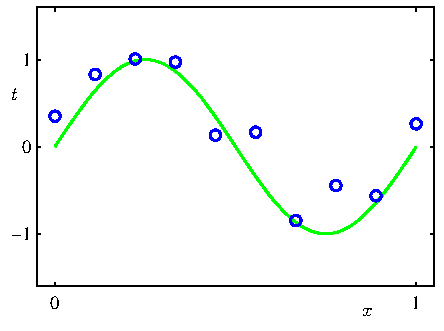
\includegraphics[width=\textwidth]{./lecture1/Figure1_2}
    \end{subfigure}%
	~
	\begin{subfigure}[b]{0.45\textwidth}
                \centering
                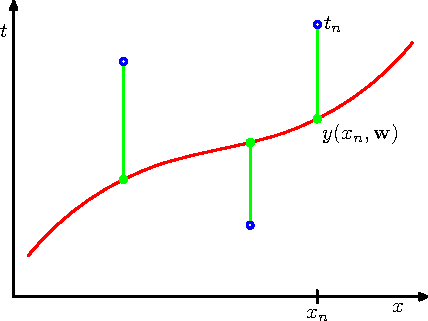
\includegraphics[width=\textwidth]{./lecture1/Figure1_3}
    \end{subfigure}%
	\caption{Figures taken from Bishop.}
\end{figure}

\begin{align*}
	y(x,w) &= w_0 + w_1x + w_2x^2 + . . . + w_Mx^M\\
	E(w) &= \sum_{n=1}^N (y(xn, w) - t_n)^2
\end{align*}

\begin{figure}
	\centering
	\begin{subfigure}[b]{0.45\textwidth}
                \centering
                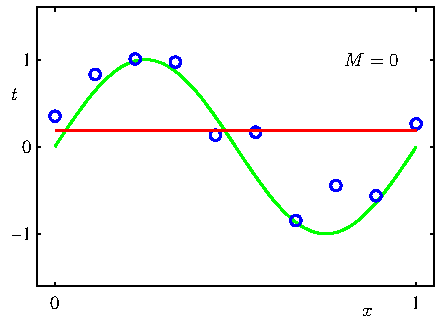
\includegraphics[width=\textwidth]{./lecture1/Figure1_4a}
    \end{subfigure}%
	~
	\begin{subfigure}[b]{0.45\textwidth}
                \centering
                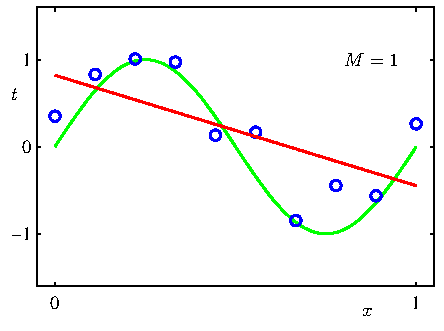
\includegraphics[width=\textwidth]{./lecture1/Figure1_4b}
    \end{subfigure}%
    
    % blank line for new line
    \begin{subfigure}[b]{0.45\textwidth}
                \centering
                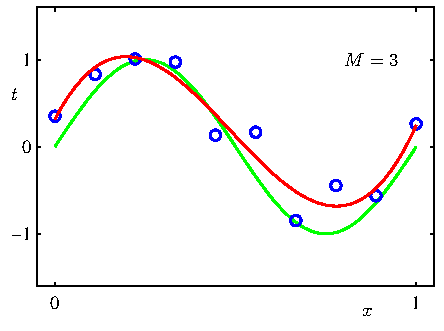
\includegraphics[width=\textwidth]{./lecture1/Figure1_4c}
    \end{subfigure}%
	~
	\begin{subfigure}[b]{0.45\textwidth}
                \centering
                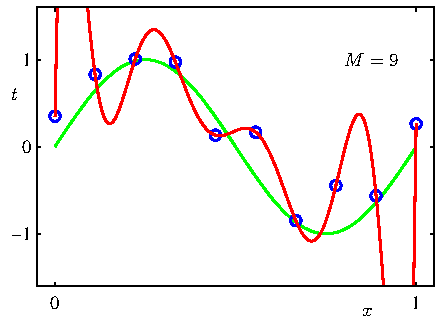
\includegraphics[width=\textwidth]{./lecture1/Figure1_4d}
    \end{subfigure}%
	\caption{Figures taken from Bishop.}
\end{figure}


\subsubsection{Generalization}
\textbf{We are interested in generalization ability. Cross-validation allows you to
quantify how well your algorithm generalizes.}\\
\begin{itemize}
	\item Split your data (randomly) into non-overlapping \textit{training} and \textit{test} sets
    \item Fit parameters on \textit{training set}
    \item Test quality of model by testing how well it fits on the test-set
    \item K-fold cross-validation: Repeat this procedure K times such that every data-point appears exactly once in a test-set.
    \item Cross-validation gives an estimate of the generalization error.
\end{itemize}

\begin{wrapfigure}{r}{0.5\textwidth}
	\centering
	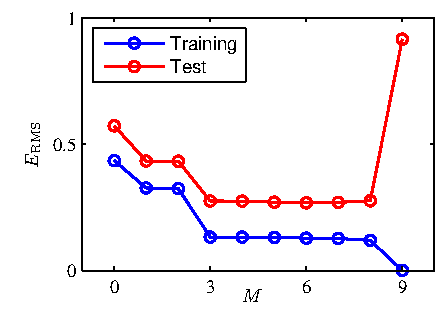
\includegraphics[width=0.45\textwidth]{./lecture1/Figure1_5}
\end{wrapfigure}

\textbf{Regularization protects against over-fitting.}\
\begin{itemize}
 \item Prefer simple explanations (=models) over complex ones: Occams Razor
 \item Trade off between model-complexity and goodness-of-fit
 \item Bayesian approach: Specify a prior distribution over models, and search for a model which both has high probability under the prior AND fits the data well
\end{itemize}

\begin{align*}
	E(w) &= \sum_{n=1}^N (y(x_n, w) - t_n)^2 + \frac{\lambda}{2} \|w\|^2
\end{align*}

\begin{figure}
	\centering
	\begin{subfigure}[b]{0.45\textwidth}
                \centering
                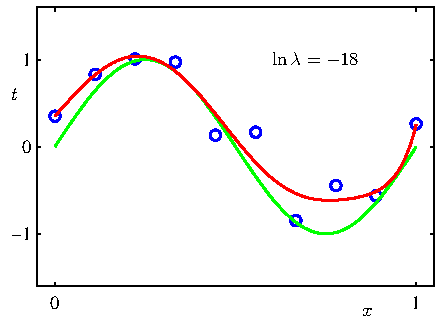
\includegraphics[width=\textwidth]{./lecture1/Figure1_7a}
    \end{subfigure}%
	~
	\begin{subfigure}[b]{0.45\textwidth}
                \centering
                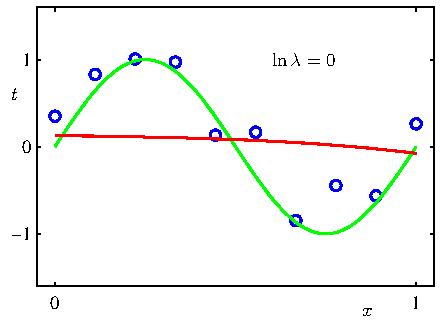
\includegraphics[width=\textwidth]{./lecture1/Figure1_7b}
    \end{subfigure}%
	\caption{Figures taken from Bishop.}
\end{figure}

\subsection{Course objective}
In this course, we follow (and promote) a very statistical (and mostly Bayesian) approach to machine learning
\begin{itemize}
	\item Many approaches in machine learning can be motivated from a statistical perspective.
	\item We will follow a statistical/probabilistic approach, but not be \textit{hard core} Bayesian
	\item Advantages of a probabilistic approach:
	\item Unified theoretical and conceptual framework
	\item Principled methods, e.g. for setting free parameters
	\item Make inferences about missing inputs
	\item Ability to sample from model
	\item Scientific reasoning: Model comparison, hypothesis testing
	\item Connections with neural coding and cognitive models
	\item Disadvantages: mostly computational in nature
	\item Exact solutions are often intractable, and an approximate solution to a great problem can be worse than a simpler approach with an exact solution
	\item \textit{Non Bayesian} algorithms are often faster and more efficient, especially on big data sets.
	\item Famous \textit{non probabilistic} algorithms: e.g. Support Vector Machines, Convolutional Neural Networks
\end{itemize}

    
    \part{Supervised Learning}
    


\documentclass[10pt, handout]{beamer}
\setbeamertemplate{navigation symbols}{}
\usefonttheme{serif} 
\usepackage{amsmath}
\usepackage{amssymb}
\usepackage{graphicx}
\usepackage{cite}
\usepackage{color} 
\usepackage{setspace}
\usepackage{hyperref}

\newcommand{\xx}{{\bf{x}}}

\begin{document}
\title{Machine Learning I Lecture III:\\ Gaussian models}   
\author{Jakob H Macke\\ Max Planck Institute for Biological Cybernetics\\ Bernstein Center for Computational Neuroscience} 
\date{XY.XY.2012} 

\frame{\titlepage} 

%\frame{\frametitle{Today: Back to basics of probability theory}} 


\frame{\frametitle{Plan for today}\tableofcontents} 

\section{Wrap up: Continuous random variables}

\frame{\frametitle{Mean, variance, and conditioning on events are the same as the discrete case, just with sums replaced by integrals.}
\begin{itemize}
\item Mean: $E(X)= \int_x x  \cdot p(x) dx$\\
\item Variance: $\mbox{Var}(X)= E(X^2)- E(X)^2$
\item Example: Uniform, Exponential [on board]
\item \pause If $X$ has pdf $p(x)$, then $X | (X \in A)$ has pdf 
\begin{align}
p_{X|A}(x)=\frac{p(x)}{P(A)}=\frac{p(x)}{\int_{x \in A} p(x) dx}
\end{align}
\item \pause Only makes sense if $P(A)>0$~!
\item Examples: Uniform, Exponential [on board]
\end{itemize}
}



\frame{\frametitle{Bivariate continuous distributions: Marginalization, Conditioning and Independence}
\begin{itemize}
\item $p_{X,Y}(x,y)$, joint probablity density function of $X$ and $Y$
\item $\int_x \int_y p(x,y)dx dy=1$
\item \pause \alert{Marginal distribution:} $p(x)= \int_{-\infty}^\infty p(x,y) dy$
\item \pause \alert{Conditional distribution:} $p(x|y)= \frac{p(x,y)}{p(y)}$ 
\item Note: $P(Y=y)=0$! Formally, conditional probability in the continuous case can be derived using infinitesimal events.
\item \pause \alert{Independence:} $X$ and $Y$ are independent if $p_{X,Y}(x,y)=p_X(x)p_Y(y)$
\end{itemize}
}

\section{Gaussians}
\frame{\frametitle{The univariate Gaussian}
\begin{align}
t &\sim \mathcal{N}(\mu,\sigma^2)\\
p(t|\mu, \sigma^2)&=\frac{1}{\sqrt{2\pi\sigma^2}}\exp\left( -\frac{1}{2}\left(\frac{t-\mu}{\sigma} \right)^2\right)
\end{align}
\begin{itemize}
\item 
The Gaussian has \alert{mean} $\mu$ and \alert{variance} $\sigma^2$ and \alert{precision} $\beta=1/\sigma^2$
\item \pause Q: What are the \alert{mode} and the \alert{median} of the Gaussian?
\item \pause Maximum Likelihood estimation of $\mu$ and $\beta$: [on board]
\item \pause Q: How would you find the conjugate prior for the Gaussian?

\end{itemize}
}


\frame{\frametitle{A (very important) aside: Products of Gaussian pdfs are (unnormalized) Gaussians pdfs}
\begin{itemize}
\item Suppose $p_1(x)=\mathcal{N}(x,\mu_1, 1/\beta_1)$ and $ p_2(x)=\mathcal{N}(x,\mu_2, 1/1\beta_2)$, then  
\pause \begin{align}
p_1(x) p_2(x) &\propto \mathcal{N}(x, \mu, 1/\beta)\\
\beta&=\beta_1+\beta_2\\
\mu&=\frac{1}{\beta}(\beta_1 \mu_1 +  \beta_2 \mu_2)
\end{align}

\pause 
In general:
\begin{align}
p_1(x) p_2(x) ... p_n(x) &\propto \mathcal{N}(x, \mu, 1/\beta)\\
\beta&=\sum_n \beta_n\\
\mu&=\frac{1}{\beta} \sum_n \mu_n \beta_n
\end{align}

\pause 
This is also true for multivariate Gaussians!

\end{itemize}
}


\section{Bayesian inference for Gaussians}

\frame{\frametitle{Bayesian Inference for the Gaussian}
\begin{itemize}
\item Suppose we are given data $D=\{x_1, \ldots, x_N\}$. 
\item We assume that the data is Gaussian-distribution with known variance $\sigma^2$ and unknown mean $\mu$.
\item Our prior for $\mu$ is Gaussian: $\mu \sim \mathcal{N}(\mu_o, \sigma^2_o)$
\item Posterior distribution over $\mu$ given the data: [on board] 
\end{itemize}
~
\pause
{\centering
\includegraphics[width=.58\textwidth]{Figure212.pdf}
\\\vspace{-.5cm}}
{\tiny[Bishop PRML Figure 2.12]}

\pause Behaviour for large $N$: [on board]
}

\frame[shrink=0]{\frametitle{What if the variance is not given?}
\begin{itemize}
\item For simplicity, assume mean to be known.
\item More convenient to work with precision $\lambda=1/\sigma^2$.
\item Conjugate prior: Gamma distribution $\mbox{Gam}(\lambda|a,b)$
\begin{align}
p(\lambda|a, b)=\frac{1}{\Gamma(a)}b^a \lambda^{a-1} exp(-b\lambda)
\end{align}
\item Posterior is $\mbox{Gam}(\lambda|a_N,b_B)$
\begin{align}
a_N &= a + \frac{N}{2}\\
b_N &= b + \frac{1}{2} \sum_{n=1}^N (x_n -\mu)^2
\end{align}
\pause
\includegraphics[width=.38\textwidth]{Figure213b.pdf}
\includegraphics[width=.38\textwidth]{Figure213c.pdf} \\\tiny[Bishop PRML Page 100]

\end{itemize}
}

\frame[shrink=0]{\frametitle{What if both the mean and the variance are unknown?}
\begin{itemize}
\item Conjugate prior: Gaussian-Gamma distribution
\begin{align}
p(\mu,\lambda) & = \mathcal{N}\left(\mu |\mu_o (\beta\lambda)^{-1}\right) \mbox{Gam}(\lambda|a,b)
\end{align}s
\includegraphics[width=.68\textwidth]{Figure214.pdf} \\\tiny[Bishop PRML Page 102]
\end{itemize}
}




 
\end{document}




    


\documentclass[10pt, handout]{beamer}
\setbeamertemplate{navigation symbols}{}
\usefonttheme{serif} 
\usepackage{amsmath}
\usepackage{amssymb}
\usepackage{graphicx}
\usepackage{cite}
\usepackage{color} 
\usepackage{setspace}
\usepackage{hyperref}

\newcommand{\xx}{{\bf{x}}}

\begin{document}
\title{Machine Learning I Lecture II:\\ Tutorial on probability theory}   
\author{Jakob H Macke\\ Max Planck Institute for Biological Cybernetics\\ Bernstein Center for Computational Neuroscience} 
%\date{\today} 

\frame{\titlepage} 

%\frame{\frametitle{Today: Back to basics of probability theory}} 


\frame{\frametitle{Plan for today}\tableofcontents} 


\section{Discrete probability distributions} 

\frame[shrink=10]{\frametitle{To specify a discrete random variable, we need a sample space and a probability mass function.}

\begin{itemize}
\item \alert{Sample space $\Omega$}: Possible 'states' $x$ of the random variable $X$ \\(outcomes of the experiment, output of the system, measurement). Examples: [on board]
\item \pause Discrete random variables either have a finite or countable number of states.
\item \pause \alert{Events:} Possible combinations of states ('subsets of $\Omega$')
\item \pause \alert{Probability mass function $P(X=x)$}: A function which tells us how likely each possible outcome is.
%\item %Rules: 
\begin{align}
P(X=x)&=P_X(x)=P(x)\\
P(x)&\geq 0 \mbox{ for each } x\\
\sum_{x \in \Omega} P(x)&=1\\
P(A) = P(x \in A) &=\sum_{x \in A} P(X=x)\\
\end{align}
\item We write: $X|q \sim \mbox{Binomial}(q)$
\item Bernoulli, Binomial, Multinonomial, Poisson:  [on board]
\end{itemize}

} 
\frame{\frametitle{Conditional probability: Updating probabilities after we obtain information.}
\begin{itemize}
\item \alert{Conditional probability:} 'Recalculated probability of event A after someone tells you that event A happened.' 
\begin{align}
P(A|B)&= \frac{P(A \cap B)}{P(B)}\\
\pause P(A \cap B)&= P(A|B) P(B)
\end{align}
\item \pause Examples: Rolls of a die
 [on board]
\item \pause Bayes Rule: 
\begin{align}
P(B|A) = \frac{P(A|B) P(B)}{P(A)}
\end{align}
\end{itemize}

}

\frame{\frametitle{Expectation and  variance characterize the mean value of a random variable and its dispersion.}
\begin{itemize}
\item Expectation (or mean): $E(X)= \sum_{x} P(X=x) x$ 
\item \pause Expectation of a function:  $E(f(X))= \sum_{x} P(X=x) f(x)$ 
\item \pause Moments= expectation of power of $X$: $M_k= E(X^k)$
\item \pause Variance: Average (squared) fluctuation from the mean
\begin{align}
 \mbox{Var}(X)&= E((X-E(X))^2)\\
 &= E(X^2)- E(X)^2\\
 &= M_2-M_1^2
\end{align}
\item \pause Standard devation: Square root of variance.
\item Illustration and examples: [on board]
\pause Aside: Difference between expectation/variance of random variable and empirical average/variance.
\end{itemize}

}


\section{Multivariate distributions: Joints, conditionals and marginals} 
\frame{\frametitle{Bivariate distributions characterize systems with two observables.}
\begin{itemize} 
\item Example [on board]     
\item \alert{Joint distribution:} $P(X=x, Y=y)$, a list of all probabilities of all possible pairs of observations
\item \pause \alert{Marginal distribution:} $P(X=x)=\sum_y P(X=x, Y=y) $
\item \pause \alert{Conditional distribution:} $P(X=x|Y=y) = \frac{P(X=x, Y=y)}{P(y=y)}$
\item \pause $X |Y$ has distribution $P(X|Y)$, where $PX(|Y)$ specifies a 'lookup-table' of all possible $P(X=x| Y=y)$
\end{itemize}
\pause
\bf Conditioning and marginalization come up in Bayesian inference ALL the time: 'Condition on what you observe. Marginalize out the uncertainty'.


}

\frame{\frametitle{The importance of conditional probabilities: Interpreting medical tests}
%P(X=aids)=.001
%P(test positive|aids)=1
%P(test positive|heality)=.001
%P(aids|positive test)= 0.091
%Sensitivity: P(test positiv |disease)
%Specificity: P(test neagative | no disease)
%100 000 People

\begin{tabular}{l|ll|l}
~ & Positive Test & Negative Test & ~\\
\hline
HIV & 475 & 25 & 500\\
no HIV & 4975 & 94525 &  99500\\
\hline
~ & 5450 &  94550 & 100000
\end{tabular}

\vspace{1cm}
[on board]
\vspace{3cm}

\tiny Source: Statistical Methods for the Social Sciences, Agresti and Finaly, Prentice Hall-- not actual data
}

 \frame{\frametitle{Expectation and covariance of multivariate distributions:}
 \begin{itemize}
\item Conditional distributions are just distributions which have a (conditional) mean or variance. 
\item \pause Note: $E(X|Y)= f(Y)$. 'If I tell you what $Y$ is, what is the average value of $X$?.
%\item $E(X,Y)= \sum_{x,y} P(X=x, Y=y) (x,y)= (E(X), E(Y))$ 
\item \pause Covariance is the expected value of the product of fluctuations: 
\begin{align}
 \mbox{Cov}(X,Y)&= E\left((X-E(X) )(Y-E(Y) )\right)\\
 &= E(XY)- E(X)E(Y)\\
 \mbox{Var(X)}&= \mbox{Cov}(X,X)
\end{align}
 \end{itemize}
\pause Aside: One common way to construct bivariate random variables is to have a random variable whos parameter is another random variable. 
 }



 \frame{\frametitle{Independence of random variables}
 \begin{itemize}
 \item Intuitively, two \alert{events are independent} if knowing that the first took places tells us nothing about the probability of the second:  $P(A|B)= P(A)$
 \item  \pause $P(A) P(B)= P(A \cap B)$
 \item \pause Two \alert{random variables} are independent if the joint p.m.f. is the product of the marginals: $P(X=x,Y=y)=P(X=x) P(Y=y)$. 
 \item If $X$ and $Y$ are independent, we write $X \perp Y$. Knowing the value of $X$ does not tell us anything about $Y$.
 \item \pause If $X$ and $Y$ are independent, $\mbox{Cov}(X,Y)=0$.
 \end{itemize}
\pause Aside: Mutual information is a measure of how 'non-independent' two random variables are.
 }



\frame{\frametitle{Multivariate distributions are the same as bivariate distributions, just with more dimensions.}
\begin{itemize} 
\item $\mathbf{X},\xx$ are vector valued.
\item Mean: $E(\mathbf{X})= \sum_{\xx} \xx P(\xx)$
\item Covariance matrix: \begin{align}
\mbox{Cov}(X_i, X_j)&= E(X_iX_j)-E(X_i) E(X_j)\\
\mbox{Cov}(\mathbf{X})&= E(\mathbf{X}\mathbf{X}^\top)-E(\mathbf{X}) 
E(\mathbf{X})^\top 
 \end{align}
\item \pause Conditional and marginal distributions: Can define and calculate any (multi or single-dimensional) marginals or conditional distributions we need:  $P(X_1)$, $P(X_1, X_2)$, $P(X_1, X_2, X_3 |X_4)$, etc..
\end{itemize}

}
\section{} 
 
 




\section{Continuous probability distributions}

\frame{\frametitle{Continous random variables}
\begin{itemize}
\item A random variable $X$ is \alert{continuous} if its sample space $X$ is uncountable. 
\item In this case, $P(X=x)=0$ for each $x$.
\item \pause If $p_X(x)$ is a \alert{probability density function} for $X$, then 
\begin{align}
P(a < X <b) &=\int_a^b p(x) dx\\
P(a<X <a+dx) \approx p(a) \cdot dx
\end{align}
\item \pause The \alert{cumulative distribution function} is $F_X(x)=P(X<x)$. We have that $p_X(x)=F'(x)$, and $F(x)=\int_{-\infty}^x p(s) ds$.
\item  \pause 
More generally: If $A$ is an event, then
\begin{align}
P(A)&=P(X \in A) =\int_{x \in A}  p(x) dx\\
P(\Omega)&=P(X \in \Omega) =\int_{x \in \Omega} p(x) dx=1
\end{align}
\item Example: Uniform, Exponential, Beta  [on board]
\end{itemize}
}



\frame{\frametitle{People will often say probability when they mean probability density.}
\begin{itemize}
\item Probability density functions do not satisfy the definitions of probability (e.g. they can bigger than $1$). However, people (including your lecturer) will often be sloppy and write things like $P(X=x)$ and say 'the probability of $X$' when they really mean 'the probability density of $X$ evaluated at $x$'.
\item \pause Similarly, people (including your lecturer) will often be sloppy and write integrals or say 'we need to integrate our $X$' when they write down general formulas-- if these formulas are applied to discrete random variables, the integrals would need to be replaced by sums.
\item \pause This might be bad practice, but it is usually clear from the context whether a random variable is discrete or continuous. In addition, it is good preparation for reading papers---many machine learning papers are very sloppy about usage of these terms.
\end{itemize}
}



\frame{\frametitle{Mean, variance, and conditioning on events are the same as the discrete case, just with sums replaced by integrals.}
\begin{itemize}
\item Mean: $E(X)= \int_x x  \cdot p(x) dx$\\
\item Variance: $\mbox{Var}(X)= E(X^2)- E(X)^2$
\item Example: Uniform, Exponential [on board]
\item \pause If $X$ has pdf $p(x)$, then $X | (X \in A)$ has pdf 
\begin{align}
p_{X|A}(x)=\frac{p(x)}{P(A)}=\frac{p(x)}{\int_{x \in A} p(x) dx}
\end{align}
\item \pause Only makes sense if $P(A)>0$~!
\item Example: Uniform, Exponential [on board]
\end{itemize}
}


%\frame{\frametitle{The univariate Gaussian}

%[on board]

%}

\frame{\frametitle{Bivariate continuous distributions: Marginalization, Conditioning and Independence}
\begin{itemize}
\item $p_{X,Y}(x,y)$, joint probablity density function of $X$ and $Y$
\item $\int_x \int_y p(x,y)dx dy=1$
\item \pause \alert{Marginal distribution:} $p(x)= \int_{-\infty}^\infty p(x,y) dy$
\item \pause \alert{Conditional distribution:} $p(x|y)= \frac{p(x,y)}{p(y)}$ 
\item Note: $P(Y=y)=0$! Formally, conditional probability in the continuous case can be derived using infinitesimal events.
\item \alert{Independence:} $X$ and $Y$ are independent if $p_{X,Y}(x,y)=p_X(x)p_Y(y)$
\end{itemize}
}

%\section{The Gaussian distribution}
 

%\frame{\frametitle{The multivariate Gaussian}

%[on board]

%}
 

%\frame{\frametitle{The magic formula: Conditional distributions in the multivariate Gaussian}

%[on board]

%}
 
\end{document}




    \section{Bayesian inference for the Gaussian distribution}

\subsection{The univariate Gaussian}
\begin{align}
t &\sim \mathcal{N}(\mu,\sigma^2)\\
p(t|\mu, \sigma^2)&=\frac{1}{\sqrt{2\pi\sigma^2}}\exp\left( -\frac{1}{2}\left(\frac{t-\mu}{\sigma} \right)^2\right)
\end{align}
\begin{itemize}
\item 
The Gaussian has \emph{mean} $\mu$ and \emph{variance} $\sigma^2$ and \emph{precision} $\beta=1/\sigma^2$
\end{itemize}

\begin{bbbox}{The univariate Gaussian}

\begin{flalign*}
	\mu = 0; \sigma^2 = 1, \\
	P(t) = \frac{1}{\sqrt{2\pi}} \mbox{e}^{-\frac{1}{2}t^2} \\
	\int_{-\infty}^{\infty} P(t) 
		&= \frac{1}{\sqrt{2\pi}} \int_{-\infty}^{\infty} \mbox{e}^{-\frac{1}{2}t^2} dt\\
		&= \frac{1}{\sqrt{2\pi}} \sqrt{2\pi} = 1
\end{flalign*}

\begin{itemize}
\item  Q: What are the \emph{mode} and the \emph{median} of the Gaussian?\\
		  Mode and median of the Gaussian are equal to the mean. This can easily be seen graphically.	
		  
\end{itemize}
\end{bbbox}

\begin{bbbox}{Maximum Likelihood estimation of $\mu$ and $\beta$}

	  \begin{align*}
	  	D &= \{ t_1 , t_2 ,\cdots , t_n \} \\
	  	L(D|\mu,\beta) &= \prod_{n=1}^N \mathcal{N} \left( t_n,\mu,\sigma^2 \right) \\
	  				   &= \sqrt{\frac{\beta}{2\pi}}^N \mbox{e}^{-\frac{\beta}{2} \sum_{n=1}^N \left(t_n - \mu\right)^2} \\
		\log L &= \frac{N}{2} \log \left( \frac{\beta}{2\pi} \right) - \frac{\beta}{2} \sum_{n=1}^N \left(t_n - \mu\right)^2 \\
		\end{align*}
		
		\text{Maximum likelihood solution for the mean } $\mu$ \\
		\begin{align*}
		0 &= \frac{\partial \log L}{\partial \mu} = -\frac{\beta}{2} \sum_{n=1}^N 2 \left(t_n - \mu \right) (-1) \\
		0 &= \sum_{n=1}^N t_n - \sum_{n=1}^N \mu \\
		\mu &= \frac{1}{N} \sum_{n=1}^N t_n \\
		\end{align*}
		
		\text{Maximum likelihood solution for the variance } $\sigma^2 = \frac{1}{\beta}$ \\
		\begin{align*}
		0 &= \frac{\partial \log L}{\partial \beta} = \frac{N}{2\beta} - \frac{1}{2} \sum_{n=1}^N 2 \left(t_n - \mu \right)^2 \\
		\sigma^2 &= \frac{1}{\beta} = \frac{1}{N} \sum_{n=1}^N 2 \left(t_n - \hat{\mu} \right)^2 \\
	  \end{align*}
Q: How would you find the conjugate prior for the Gaussian? \\

\end{bbbox}

\textbf{(very important) aside: Products of Gaussian pdfs are (unnormalized) Gaussians pdfs}
\begin{itemize}
\item Suppose $p_1(x)=\mathcal{N}(x,\mu_1, \frac{1}{\beta_1})$ and $ p_2(x)=\mathcal{N}(x,\mu_2, \frac{1}{\beta_2})$, then  
 \begin{align}
p_1(x) p_2(x) &\propto \mathcal{N}(x, \mu, 1/\beta)\\
\beta&=\beta_1+\beta_2\\
\mu&=\frac{1}{\beta}(\beta_1 \mu_1 +  \beta_2 \mu_2)
\end{align}

\begin{bbbox}{Products of Gaussians}
	Quadratic form for the Gaussian:
	\begin{align*}
		p(t|\mu, \sigma^2) 
		&=\frac{1}{\sqrt{2\pi\sigma^2}}\exp\left( -\frac{1}{2}\left(\frac{t-\mu}{\sigma} \right)^2\right) \\
		&= \frac{1}{Z} \exp \left( \underbrace{a}_{-\frac{1}{2}\text{precision}}x^2 + \underbrace{b}_{\text{precision} \times \text{mean}}x \right) \\
	\end{align*}
	
	We show that the product of two Gaussians $p_1(x)$ and $p_2(x)$ is again Gaussian: \\
	\begin{align*}
	p_1(x) &= \frac{1}{Z_1} \exp \left( -\frac{\beta_1}{2} \left(x-\mu_1 \right)^2 \right) 	\\
	p_2(x) &= \frac{1}{Z_2} \exp \left( -\frac{\beta_2}{2} \left(x-\mu_2 \right)^2 \right) 	\\
	p_1(x) p_2(x) &= \frac{1}{Z_s} \exp \left( -\frac{\beta_1}{2} \left( x - \mu_1 \right)^2
					  -\frac{\beta_2}{2} \left( x - \mu_2 \right)^2	\right)\\
				  &= \frac{1}{Z_q} \exp \left( -\left( \frac{\beta_1}{2} + \frac{\beta_2}{2}\right) x^2
	                 + 2\left( \frac{\beta_1}{2} \mu_1 + \frac{\beta_2}{2} \mu_2 \right) x \right)\\
	\beta &= \beta_1 + \beta_2 \\
	\beta \mu &= = \beta_1 \mu_1 + \beta_2 \mu_2 \\
	\mu &= \frac{1}{\beta} \left( \beta_1 \mu_1 + \beta_2 \mu_2 \right)
	\end{align*}
	The quadratic form helps us to simply read out the parameters of our resulting Gaussian. We will see later that this observation comes in handy for Bayesian inference with Gaussians.
\end{bbbox}
 
In general:
\begin{align}
p_1(x) p_2(x) ... p_n(x) &\propto \mathcal{N}(x, \mu, 1/\beta)\\
\beta&=\sum_n \beta_n\\
\mu&=\frac{1}{\beta} \sum_n \mu_n \beta_n
\end{align}

 
This is also true for multivariate Gaussians!

\end{itemize}



\subsection{Bayesian inference for Gaussians}

\begin{itemize}
\item Suppose we are given data $D=\{x_1, \ldots, x_N\}$. 
\item We assume that the data is Gaussian-distribution with known variance $\sigma^2$ and unknown mean $\mu$.
\item Our prior for $\mu$ is Gaussian: $\mu \sim \mathcal{N}(\mu_o, \sigma^2_o)$
\item Posterior distribution over $\mu$ given the data: [on board] 
\end{itemize}

\begin{bbbox}{Posterior inference for the Gaussian}
	Here we want to derive the posterior  distribution for the mean of a Gaussian. For now we will assume that the variance $\sigma^2$ of our Gaussian is known and that the only parameter of interest is $\mu$. \\
	We define a prior over $\mu$:   $p(\mu) = \mathcal{N}(\mu_0, \sigma^2_0)$ which is again Gaussian. \\
	From before we know that our posterior distribution over $\mu$ is again Gaussian:
	\begin{align*}
		p(\mu|\sigma^2, \underbrace{\mu_0, \sigma_0^2}_{Prior},D)	
		            &\propto p(D|\mu,\sigma^2,\mu_0, \sigma_0^2) p(\mu|\mu_0, \sigma_0^2) \\
		            &\propto \prod_{n=1}^N \mathcal{N}(x_n,\mu,\sigma^2) \mathcal{N}(\mu,\mu_0, \sigma_0^2) \\
		            &\propto \mathcal{N}(\mu,\mu_{post},\sigma_{post}^2) \\
		\frac{1}{\sigma_{post}^2} &= \sum_{n=1}^N \left(\frac{1}{\sigma^2} \right) + \frac{1}{\sigma_0^2} \\
		\sigma_{post}^2 &= \frac{1}{\frac{N}{\sigma^2} + \frac{1}{\sigma_0^2}} \\
		\mu_{post} &= \sigma_{post}^2 \left( \sum_{n=1}^N \left( x_n\frac{1}{\sigma^2} \right) + \mu_0 \frac{1}{\sigma_0^2} \right)
	\end{align*}
	
Behaviour for large $N$: [on board]
\begin{align*}
	\text{for large N: } \sigma_{post}^2 = \frac{\sigma^2}{N} \\
	\mu_{ML} &= \frac{1}{N} \sum_{n=1}^N x_n \\
	\mu_{post} &= \frac{\left( \sum_{n=1}^N \left( x_n\frac{1}{\sigma^2} \right) + \mu_0 \frac{1}{\sigma_0^2} \right)}{\frac{N}{\sigma^2} + \frac{1}{\sigma_0^2}} \\
	N \rightarrow \infty: &\mu_{post} = \mu_{ML} \\
	\sigma_0^2 \rightarrow 0: &\mu_{post} = \mu_{ML} \\
\end{align*}

\end{bbbox}

\begin{figure}
	\centering
	\includegraphics[width=.5\textwidth]{./lecture4/Figure212.pdf}
	\caption{Bishop Figure 2.12}
\end{figure}

\subsubsection{What if the variance is not given?}
\begin{itemize}
\item For simplicity, assume mean to be known.
\item More convenient to work with precision $\lambda=1/\sigma^2$.
\item Conjugate prior: Gamma distribution $\mbox{Gam}(\lambda|a,b)$
\begin{align}
p(\lambda|a, b)=\frac{1}{\Gamma(a)}b^a \lambda^{a-1} exp(-b\lambda)
\end{align}
\item Posterior is $\mbox{Gam}(\lambda|a_N,b_B)$
\begin{align}
a_N &= a + \frac{N}{2}\\
b_N &= b + \frac{1}{2} \sum_{n=1}^N (x_n -\mu)^2
\end{align}

\begin{figure}
\centering
\begin{subfigure}[b]{0.45\textwidth}
                \centering
                \includegraphics[width=\textwidth]{./lecture4/Figure213b.pdf}
    \end{subfigure}%
	~
	\begin{subfigure}[b]{0.45\textwidth}
                \centering
                \includegraphics[width=\textwidth]{./lecture4/Figure213c.pdf}
    \end{subfigure}%
   	\caption{Gamma distribution with different parameterizations. The Gamma distribution is a conjugate prior for the presision of a Gaussian. Figures taken from Bishop page 100.}
	
\end{figure}
\end{itemize}


\subsubsection{What if both the mean and the variance are unknown?}
\begin{figure}[h]
	\centering
		\includegraphics[width=0.7\textwidth]{./lecture4/Figure214.pdf}
		\caption{The Gaussian-Gamma distribution, a conjugate prior for mean and precision of a Gaussian. Bishop figure 2.14, page 102.}
\end{figure}    
\begin{itemize}
\item Conjugate prior: Gaussian-Gamma distribution
\begin{align}
p(\mu,\lambda) & = \mathcal{N}\left(\mu |\mu_o (\beta\lambda)^{-1}\right) \mbox{Gam}(\lambda|a,b)
\end{align}
\end{itemize}

    \section{Bayesian linear regression}

\subsection{Linear regression revisited}
\begin{itemize}
\item Suppose that we have data $D=\{(\xx_1, t_1), \ldots, (\xx_N, t_N) \}$
\item We assume that the data can be modelled by some function $t_n \approx y(x, \omega)+ \epsilon$, where $\epsilon$ models additive noise.
\item  We assume that noise is independent, identically distributed and Gaussian: 
\begin{align}
	\epsilon &\sim \mathcal{N}(0,\beta^{-1})\\
	t|\xx, \omega, \beta &\sim \mathcal{N}(y(\xx,\omega), \beta^{-1})
\end{align}
\end{itemize}

\begin{figure}
	\centering
	\includegraphics[width=.5\textwidth]{./lecture5/Figure128.pdf}
	\caption{Linear regression. Bishop Fgure 1.28}
\end{figure}


\subsection{Maximum likelihood estimation for linear regression}
\begin{itemize}
\item We consider a linear model $y(\xx,\omega)= \omega^\top \xx$
\item ~[On board: Likelihood, Maximum Likelihood Solution, Predictive distribution from MLE]\\
\item  For a Bayesian treatment, we need priors.
\end{itemize}

\begin{bbbox}{Maximum likelihood estimation for linear regression}
	\begin{align*}
			L(t | x,\omega) &= \log \left( \prod_{n=1}^N p(t_n |  x_n, \omega ) \right) \\
			        &= \sum_{n=1}^N \log \left( \frac{1}{\sqrt(2\pi)} \exp \left( - \frac{\beta}{2} \left( t_n - 	\omega^{\top} x_n \right)^2 \right) \right) \\
			        &= const. + \sum_{n=1}^N - \frac{\beta}{2} \left( t_n - \omega^{\top} x_n \right)^2 \\
			        &= const - \underbrace{\frac{\beta}{2} \sum_{n=1}^N \left( t_n - \omega^{\top} x_n \right)^2}_{AMSE - average mean squared error} \\
	   \hat{\omega} &= \left( \sum_{n=1}^N x_n x_n^{\top} \right)^{-1} \left( \sum_{n=1} x_n t_n \right) \\			 	    \end{align*}
	Predictive distribution \\
	$P(t^{*} | x^{*},0) = P(t^{*} | x^{*},\hat{\omega}) = \mathcal{N}(\omega^{\top} x^{*}, \frac{1}{\beta})$ 
\end{bbbox}

\subsection{Maximum a posteriori estimation for the linear regression.}
\begin{align}
\omega_i &\sim \mathcal{N}(0,\alpha^{-1})\\
p(\omega| \alpha) &= \prod_{i=1}^M  \sqrt{\frac{\alpha}{{2\pi}}}\exp\left( -\frac{\alpha}{2}  {\omega_i^2}\right)\\
&%
 =\left(\frac{\alpha}{2\pi}\right)^{M/2} \exp \left(-\frac{\alpha}{2} \omega^\top \omega  \right) \\
 \text{where } \forall i,j: \alpha_i &= \alpha_j
\end{align}

\begin{bbbox}{Finding the maximum-a-posteriori of $\omega$}
	\begin{align*}
		L_{post}(t | x,\omega) &= \log \left( \prod_{n=1}^N p(t_n |  x_n, \omega ) p(\omega|\alpha)\right) \\
		 &= \sum_{n=1}^N \log \left( \frac{1}{\sqrt(2\pi)} \exp \left( - \frac{\beta}{2} \left( t_n - 	\omega^{\top} x_n \right)^2 \right) \frac{\alpha}{2\pi}^{\frac{M}{2}} \exp \left( -\frac{\alpha}{2} \omega^{\top}\omega \right) \right) \\
		 &= const. - \frac{\beta}{2} \sum_{n=1}^N \left( t_n - \omega^{\top} x_n \right)^2 -\frac{\alpha}{2} \omega^{\top}\omega \\
	\hat{\omega} &= \left( \sum_{n=1}^N x_n x_n^{\top} + \frac{\alpha}{\beta} \mathbf{I}_M \right)^{-1} \left( \sum_{n=1} x_n t_n \right) \\			 
	\end{align*}
\end{bbbox}


\subsection{Basis functions in linear regression}
\textbf{If you are smart about choosing good basis functions ('features'), linear regression can get you pretty far.}
\begin{itemize}
\item If we use nonlinear basis functions $\phi(x)$, can model nonlinear relationships with $y(\omega, \xx)= \omega^\top \phi(x)$.
\item Polynomial regression: $\phi(x)=(1,x,x^2,x^3)$ ; (cubic feature space) 
\item 'Gaussian bumps': $\phi_i(x)= \exp\left((x-s_i)^2/\sigma_i^2 \right)$
\item Sigmoids $\phi_i(x)=1/(1+\exp(-x-s_i))$
\item  'Kernel methods' are essentially linear algorithms which take one basis function per data-point.
\item Predictive Mean [on board]
\end{itemize}

\begin{figure}
\centering
	\begin{subfigure}[b]{0.3\textwidth}
                \centering
                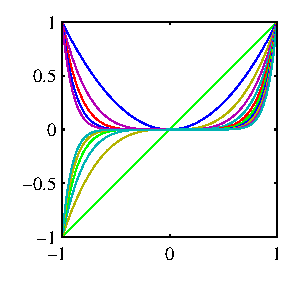
\includegraphics[width=\textwidth]{./lecture5/Figure31a.pdf}
                \caption{Polynomial basis.}
    \end{subfigure}%
	~
	\begin{subfigure}[b]{0.3\textwidth}
                \centering
                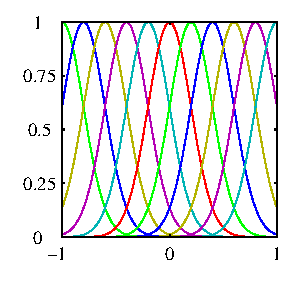
\includegraphics[width=\textwidth]{./lecture5/Figure31b.pdf}
                \caption{Gaussian bumps.}
    \end{subfigure}%
	~
	\begin{subfigure}[b]{0.3\textwidth}
                \centering
                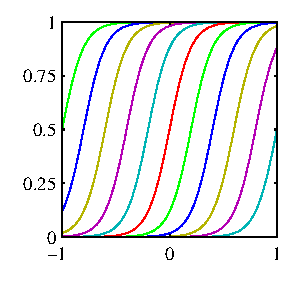
\includegraphics[width=\textwidth]{./lecture5/Figure31c.pdf}
                \caption{Logistic sigmoids.}
    \end{subfigure}%
    \caption{Non-linear basis functions.}
\end{figure}


\subsection{Bayesian linear regression}


\textbf{Bayesian linear regression takes into account our uncertainty about parameters.}

\begin{itemize}
\item Posterior distribution is Gaussian $\rightarrow$ Posterior mean and MAP coincide!
\item  However, neither the MLE nor the MAP solution take into account that we have (posterior) uncertainty about the parameters
\end{itemize}


\begin{figure}
\centering
	\begin{subfigure}[b]{0.45\textwidth}
		\centering	
		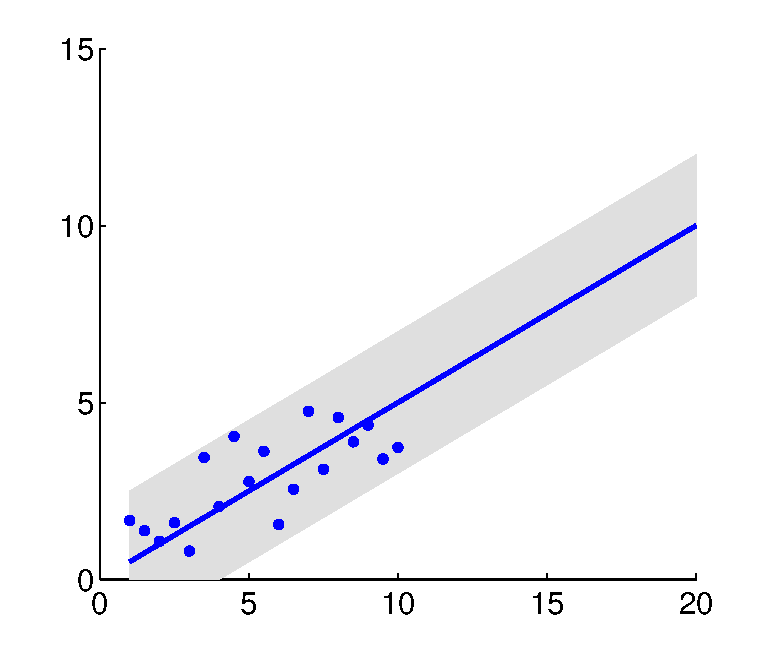
\includegraphics[width=\textwidth]{./lecture5/LinReg.pdf}
	\end{subfigure}
	~
	\begin{subfigure}[b]{0.45\textwidth}
		\centering
		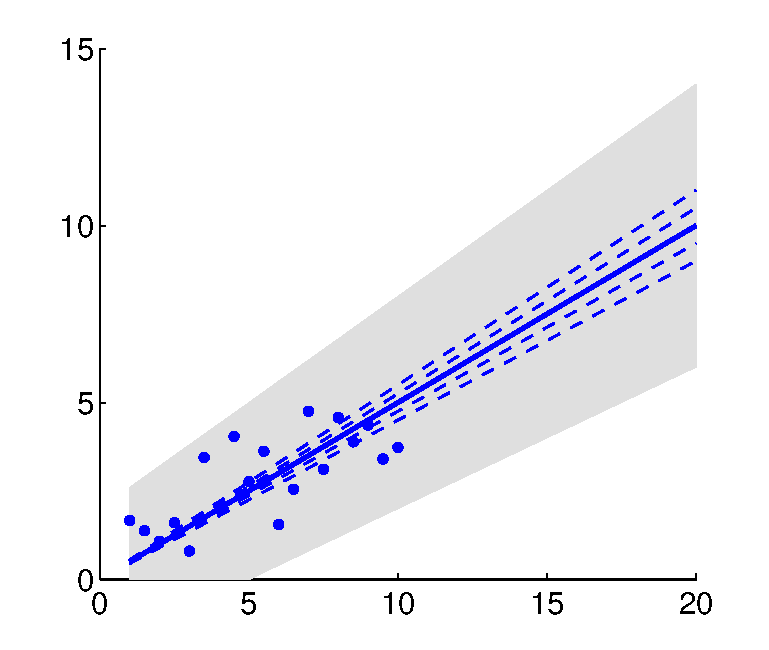
\includegraphics[width=\textwidth]{./lecture5/LinRegBayes.pdf}
	\end{subfigure}
\end{figure}


\subsection{Gaussian processes}
\textbf{Illustration: Climate prediction [by Carl Rasmussen, University of Cambridge, using Gaussian Processes]}

\begin{figure}
	\centering
	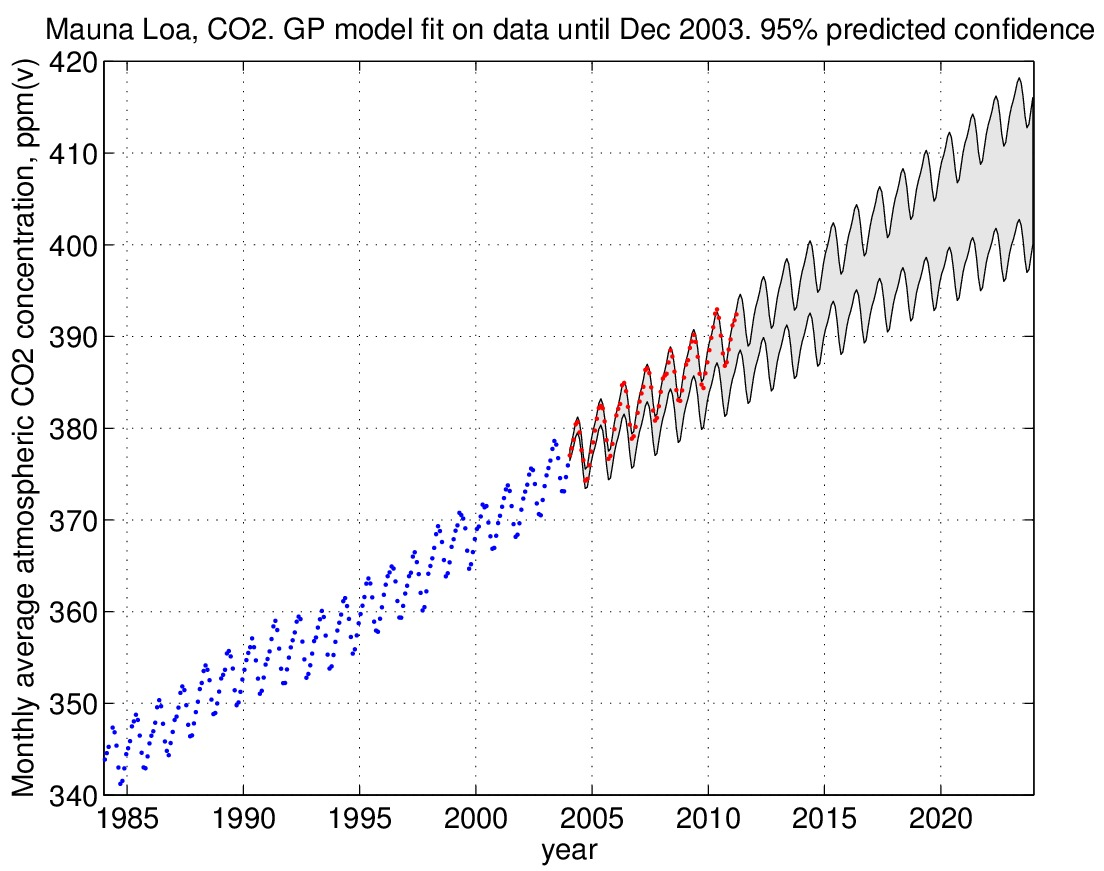
\includegraphics[width=0.5\textwidth]{./lecture5/Rasmussen2}
	\caption{Gaussian process regression.}
\end{figure}


\subsection{Sequential update of the posterior distribution}
\textbf{Bayesian regression illustrated: The more data we observe, the more constrained the parameters are.}

\begin{figure}
	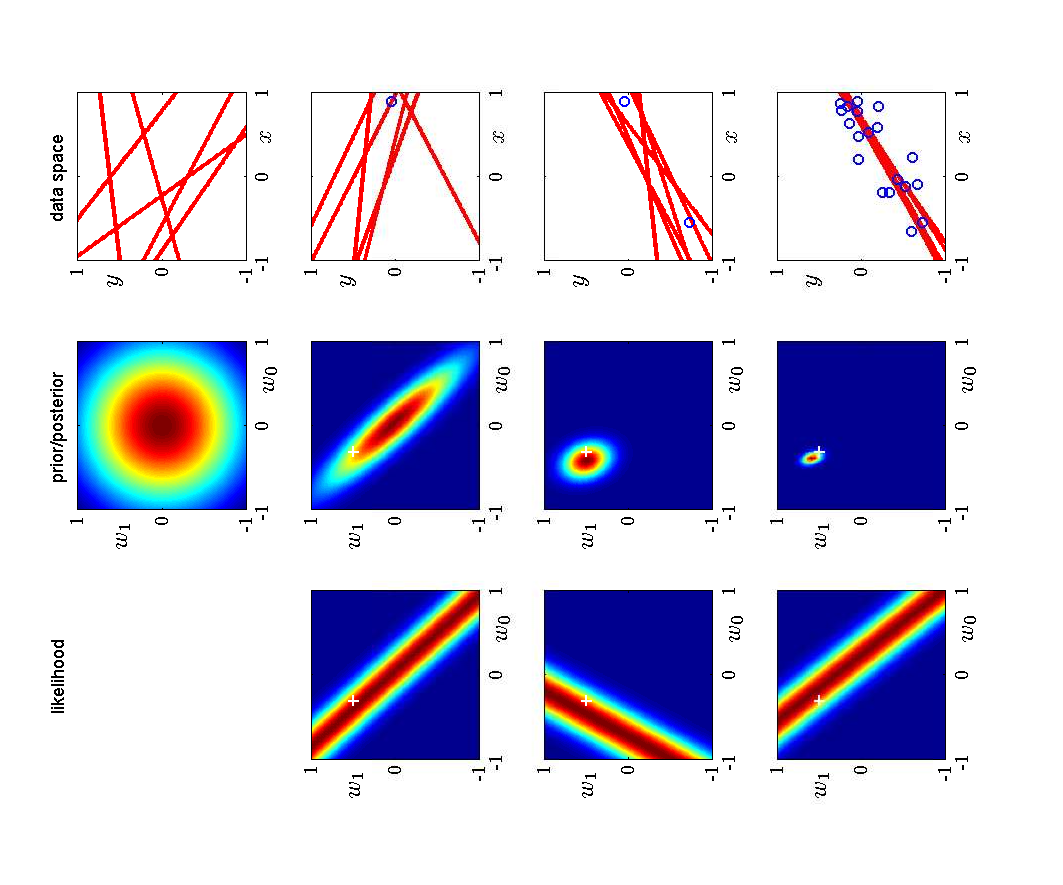
\includegraphics[width=\textwidth]{./lecture5/Figure37.pdf}
	\caption{Sequential update of the Gaussian posterior.}
\end{figure}



\textbf{Calculating the predictive mean and variance for Bayesian regression}

Assume $\alpha$ and $\beta$ as given.\\ Posterior distribution: [derivation on board]

\begin{bbbox}{Bayesian linear regression: calculating posterior mean and variance}
	Recall the quadratic form for the Gaussian: \\
	\begin{align*}
		&\frac{1}{Z} \exp \left( -\frac{1}{2} \left( x-\mu \right)^{\top} \Sigma^{-1} \left( x-\mu \right) \right) \\
		           &= \frac{1}{Z} \exp \left( -\frac{1}{2} \left( x^{\top}\Sigma^{-1}x + \mu^{\top}\Sigma^{-1}\mu 
		             - \mu^{\top}\Sigma^{-1}x - x^{\top}\Sigma^{-1}\mu \right) \right)\\
		           &= \frac{1}{Z} \exp \left( -\frac{1}{2} x^{\top}\Sigma^{-1}x + x^{\top}\Sigma^{-1}\mu + const. \right) \\
	\end{align*}
	Here again we can easily read out the posterior mean and covariance from the two terms. \\
	We say that $\omega | D \sim \mathcal{N}\left( \mu_{post}, \Sigma_{post}\right)$. \\
	Since the mode and mean of a Gaussian are the same thing we already know from our MAP estimation that:
	$ \mu_{post} = \left( \sum_{n=1}^N x_n x_n^{\top} + \frac{\alpha}{\beta} \mathbf{I}_M \right)^{-1} \left( \sum_{n=1} x_n t_n \right)$ \\
	The next thing we have to do is to bring the posterior  distribution into the quadratic form from above and to read out the posterior covariance. Note that all terms that are independents from $\omega$ will sucked into the constant term: \\
	\begin{align*}
		P(\omega|D) &= \frac{1}{Z_1} \prod_{n=1}^N P(t_n|x_n,\omega) P(\omega) \\
		&= \frac{1}{Z_2} \exp \left( \sum_{n=1}^N -\frac{\beta}{2} \left( \omega^{\top} x_n - t_n \right) ^2 - \frac{\alpha}{2} \omega^{\top} \omega \right) \\
		&= \frac{1}{Z_2} \exp \left( -\frac{\beta}{2} \sum_{n=1}^N \left( \omega^{\top} x_n - t_n \right) \left( \omega^{\top} x_n - t_n \right)^{\top} - \frac{\alpha}{2} \omega^{\top} \omega \right) \\
		&= \frac{1}{Z_3} \exp \left( -\frac{1}{2} \left( \beta \sum_{n=1}^N \omega^{\top} x_n x_n^{\top} \omega + \alpha \omega^{\top} \omega \right) \right) \\
		&= \frac{1}{Z_3} \exp \left( -\frac{1}{2} \left( \omega^{\top} \left( \beta \sum_{n=1}^N x_n x_n^{\top} + \alpha \mathbf{I}_M \right) \omega \right) \right) \\
		\Sigma_{post}^{-1}&=\alpha \mathbf{I}_M + \beta \sum_{n=1}^N x_n x_n^\top\\
	\end{align*}
\end{bbbox}

\begin{align}
\Sigma_{post}^{-1}&=\alpha \mathbf{I}+\beta \sum_i x_i x_i^\top\\
\mu_{post}&=\Sigma_{post} \beta \sum_i x_i t_i
\end{align}

Predictive distribution: [derivation on board]

\begin{bbbox}{Predictive distribution}
	We note that in the case of a regression the predictive error arises from our uncertainty about the parameters as well as the variance which is inherent to our predicted variable. We want to calculate the predictive distribution starting from the observation that making a prediction is basically a concatenation of two random variables.
	\begin{align*}
		t^* &| D, x_*: \;
		t^* = \underbrace{\omega^{\top}x_*}_{y^*} + \epsilon \\		
%		\mu &\sim \mathcal{N}(\mu_0, \frac{1}{\tau}); \;
%		x|\mu \sim \mathcal{N}(\mu,\frac{1}{\beta}); \;
%		\rightarrow x \sim \mathcal{N}(\mu_0, \frac{1}{\tau} + \frac{1}{\beta}) \\
		y^* &\sim \mathcal{N} (\mu_*,\frac{1}{\tau_{*}}); \;
		t^*|y^* \sim \mathcal{N}(y^*,\frac{1}{\beta}); \;
		\rightarrow \underbrace{t^* \sim \mathcal{N}(\mu_*,\frac{1}{\tau_{*}} + \frac{1}{\beta})}_{\text{Predictive distribution}} \\
	\end{align*}
	
We see that the variance of our predictive distribution is calculated from the variance in our parameter estimate and from the variance in $t$. We can further express the posterior distribution based on:
	\begin{align*}
		\mu_* &= E(y^* | D) = E(\omega^{\top} x_* | D) \\
		      &= E(\omega^{\top} | D) x_* = E(\omega | D)^{\top} x_* \\
		      &= \mu_{post}^{\top} x_* \\
		\frac{1}{\tau_{*}} &= \mbox{Var}(y^* | D) \\
		     &= \mbox{Var}(\omega^{\top} x_* | D) = x_*^{\top} \mbox{Var}(\omega^{\top} | D) x_* \\
   		     &= x_*^{\top} \Sigma_{post} x_* \\
	\end{align*}
\end{bbbox}

\begin{align}
E(t^*|D,x^*)&= \mu_{post}^\top x^* \\
\mbox{Var}(t^*|D,x^*)&=  1/\beta+ x^{*\top} \Sigma_{post} x^*
\end{align}
What if there are basis functions? [on board]



\subsection{Fully Bayesian linear regression}


\textbf{But, where do we get $\alpha$ and $\beta$ from?}

\begin{itemize}
\item Bad news: Getting these makes things more complicated.
\item  Good news: This will not be on the exam (unless I take that back explicitly...). 
\item  'Full' Bayesian inference: Integrate out $\alpha$, $\beta$. No closed form solution. Use (e.g.) variational inference.
\item  Practical solution: optimize $\alpha$ and $\beta$ by \emph{maximizing the evidence}, also known as \emph{marginal likelihood} or \emph{likelihood type 2}
\begin{align}
E&=\log P(\alpha, \beta|D)\\
&= \log \int_\omega p(D|\omega,\beta) p(\omega|\alpha) p(\alpha,\beta)    d \omega\\
&= \frac{M}{2}\log(\alpha)+\frac{N}{2}\log \beta-\mbox{M}(\mu_{post})+\frac{1}{2}|\Sigma_{post}|-\frac{N}{2} \log(2\pi) 
\end{align}
\item $\mu_{post}$ and $\Sigma_{post}$ are the posterior mean and covariance, and $\mbox{M}(\mu_{post})=\frac{\beta}{2}\sum_n (t_n-y(\mu_{post},\xx_n))^2+\frac{\alpha}{2} \mu_{post}\mu_{post}^\top$ is the quadratic cost function evalulated at the posterior mean (see Bishop 3.5 for details).
\end{itemize}


\textbf{Optimization of the marginal likelihood is a Bayesian alternative to parameter-setting by cross-validation.}

\textbf{What we have not had time to cover:}
\begin{itemize}
\item \emph{Non-Gaussian priors:} The most important non-Gaussian prior is the `Laplace prior' ('L1 regularization'), which leads to sparse MAP-solutions.
\item \emph{Non-Gaussian noise models:} If you know that your noise is not Gaussian but, say, Poisson, use 'generalized linear regression'. Some choices of noise models are more robust to outliers than the Gaussian. We will do one specific example of generalized linear regression in the last lecture.
\item \emph{Nonlinear regression models:} The most important Bayesian nonlinear regression technique is \emph{Gaussian process regression}. In a nutshell, GP regression is like linear regressions but the algorithm puts ne basis function at each data-point. To understand GP regression, you need to understand Gaussians.
\end{itemize}



    


\documentclass[10pt, handout]{beamer}
\setbeamertemplate{navigation symbols}{}
\usefonttheme{serif} 
\usepackage{amsmath}
\usepackage{amssymb}
\usepackage{graphicx}
\usepackage{cite}
\usepackage{color} 
\usepackage{setspace}
\usepackage{hyperref}

\newcommand{\xx}{{\bf{x}}}

\begin{document}
\title{Machine Learning I Lecture VI:\\ Linear models for Classification}   
\author{Jakob H Macke\\ Max Planck Institute for Biological Cybernetics\\ Bernstein Center for Computational Neuroscience} 
\date{XY.XY.2012} 

\frame{\titlepage} 

%\frame{\frametitle{Today: Back to basics of probability theory}} 


\frame{\frametitle{Plan for today}\tableofcontents} 

\section{Binary classification}
\frame{\frametitle{Binary Classification: Assign each data point to one of two classes.} 

%\multicolumn
\begin{columns}
\begin{column}{4cm}
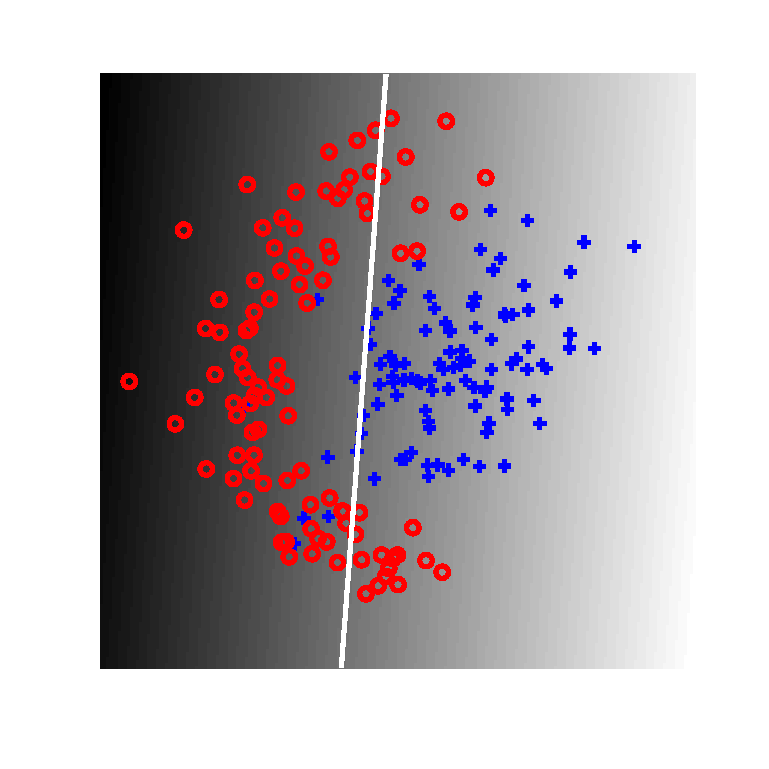
\includegraphics[width=1.1\textwidth]{LinClassification.pdf}
\end{column}
\begin{column}{7.5cm}
Examples:
\begin{itemize}
 \item Is there a face in this image?
\item Will this neuron spike in response to this stimulus?
\item Based on this brain-scan, does this patient have a given disease or not?
\item  Will this customer buy this product or not?
\item Is this person likely to be a democrat/republican? 
\end{itemize}
%\item
 \pause Notation: we have data $D=\{(x_1, t_1),\ldots, (x_N, t_N)\}$, with $t_n=1$ if $x_n$ belongs to class $1$ and $t_n=-1$ if $x_n$ belongs to class $-1$.
\end{column}
\end{columns}
}





\frame{\frametitle{We focus on linear decision rules, also known as `linear discriminant functions'.} 

%\multicolumn

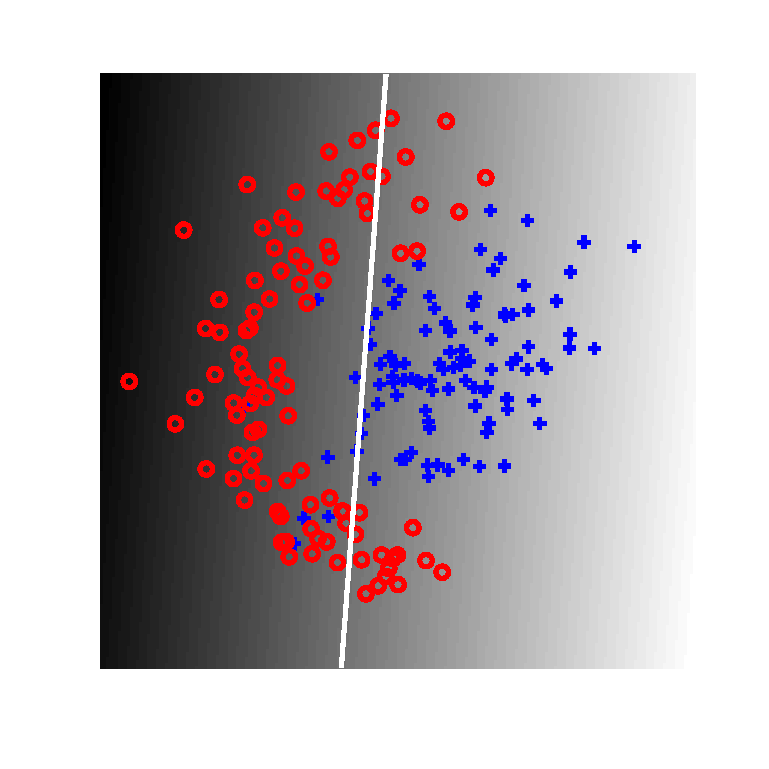
\includegraphics[width=.5\textwidth]{LinClassification.pdf}
\pause
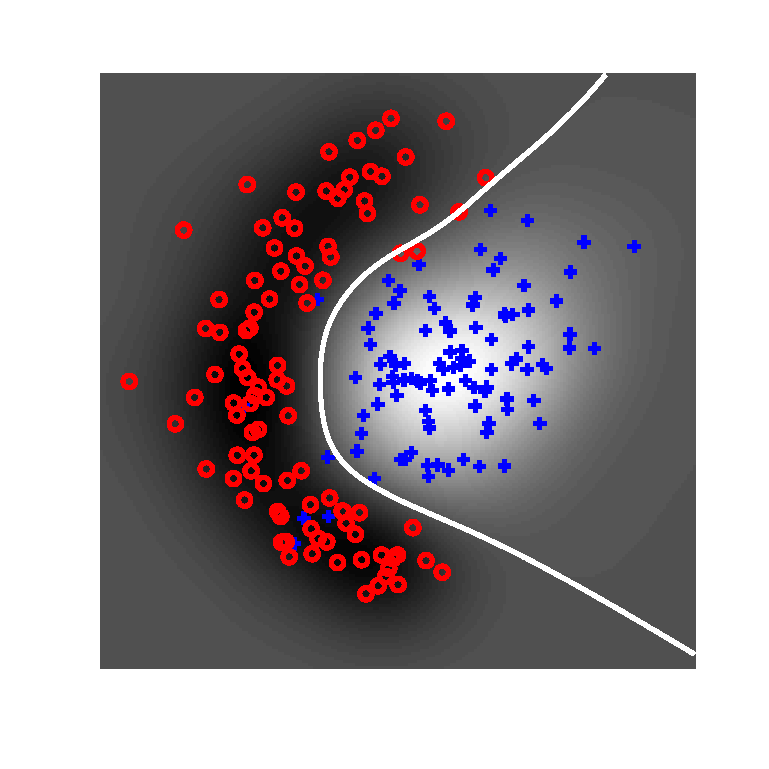
\includegraphics[width=.5\textwidth]{NonLinClassification.pdf}

\pause 

Of course, linear algorithms can be used together with \alert{nonlinear feature spaces} or \alert{nonlinear basis functions} in order to solve nonlinear classification problems!
}

\frame{\frametitle{Linear discriminants separate the space by a hyperplane, and the parameters define its normal vector.} 

%\multicolumn


%\includegraphics[width=.4\textwidth]{LinearSeparators.pdf}
\begin{itemize}
\item Decision function: $y(\xx)=\omega^\top \xx + \omega_o$
\item \pause Classification: \begin{align}
\mbox{if~}y(\xx)>0 & \mbox{~say $\xx$ belongs to class 1}\\
\mbox{if~}y(\xx)<0 & \mbox{~say $\xx$ belongs to class -1}\\
 \end{align}
\item The decision-surface has equation $y(\xx)=0$, and is a hyperplane of dimensionality $D-1$.
\item \pause $\omega$ is the normal vector to the plane, and points into the positive class.
\item \pause $\omega_o$ determines the location of the decision-surface
\item \pause $|y(\xx)|$ is proproptional to the perpendicular distance to the decision-surface (with factor $1$ if $|| \omega ||=1$).
\end{itemize}

}

\frame{\frametitle{Multiple algorithms and methods exist for finding a good $\omega$.} 
\begin{itemize}
\item Mis-classification rate $C(\omega)= \frac{1}{N} \sum_n \delta\left[y(\xx_n) =t_n\right]$ (i.e. average number of errors) difficult to optimize over $\omega$, and might have multiple solutions.
\item \pause Many algorithms can be derived by replacing $C$ by another cost-function which can be optimized.
\item \pause Linear classification algorithms include Least-square classification, Fisher's linear Discriminant, Logistic regression, Support Vector Machines and Rosenblatts' perceptron.
\end{itemize}
}

\section{Least Square Classification}
\frame{\frametitle{You already know one algorithm for linear classification: least square classification.} 
\begin{itemize}
\item We have to fit the function $y(\xx)= \omega^\top \xx+ \omega_o $ to data.
\item \pause Simply do a linear regression from $\xx$ to $t$ by minimizing the sum-of-squared errors $\sum_n (y(\xx_n)-t_n)^2$.
\item \pause $\omega_{reg}=  \left(\sum_n x_n x_n^\top  \right)^{-1} \sum_n x_n t_n$
\item \pause Q: In what situations might this be a bad idea?
\end{itemize}
\pause
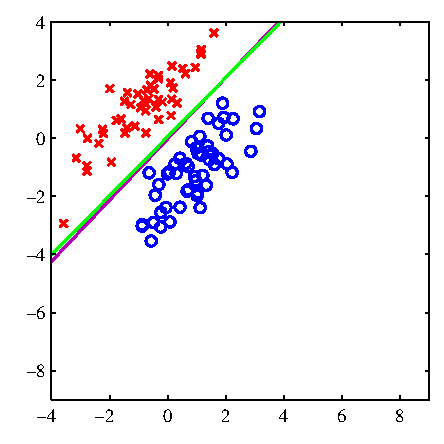
\includegraphics[width=.4\textwidth]{Figure44a.pdf}
\pause
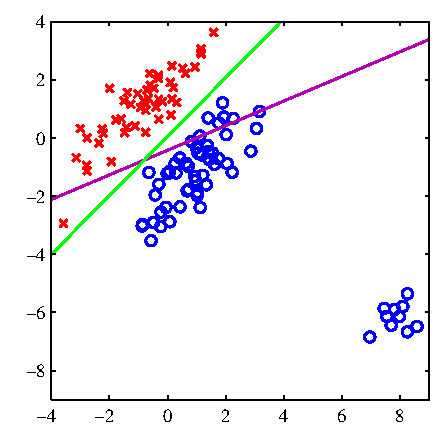
\includegraphics[width=.4\textwidth]{Figure44b.pdf}
\\
\tiny Bishop PRML Figure 4.4
}


\section{Fisher's linear discriminant}
\frame[shrink=5]{\frametitle{'Fisher's linear discriminant' is a classical and simple algorithm for linear classification} 
\begin{columns}
\begin{column}{3.5cm}

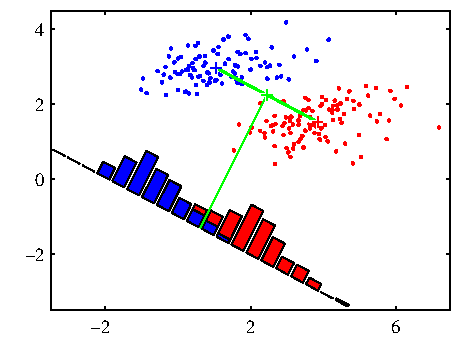
\includegraphics[width=1.2\textwidth]{Figure46a.pdf}

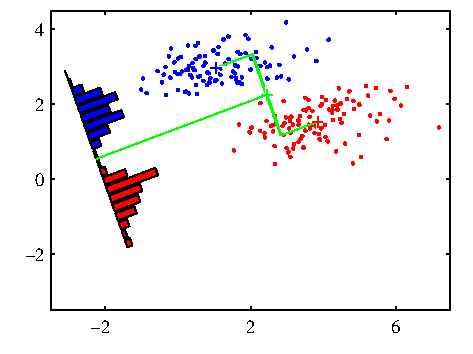
\includegraphics[width=1.2\textwidth]{Figure46b.pdf}

~\\
\tiny Bishop PRML Figure 4.6
\end{column}
\begin{column}{7.5cm}
\begin{itemize}
\item $\mathbf{m_+}= \frac{1}{N_+}\sum_{n \in C_+} x_n$ \hspace{.5cm} $\mathbf{m_{-}}= \frac{1}{N_-}\sum_{n \in C_{-}} x_n$ 
\item \pause Maximize projection-distance of class means 
[projected mean/variance: on board]
$\omega_{simple} \propto \mathbf{m}_+-\mathbf{m}_-$ 
\item \pause Maximizing distance between means ignores that the projected variances might also be big. 
\item \pause Fix:  Maximize the ratio of between-class variance to within-class variance ('signal to noise'). Fisher criterion
\begin{align}
J_\omega = 2\frac{(m_+-m_-)^2}{s_+^2+s_-^2}
\end{align}
[Details and solution: on board]
%\item 
\pause 
$\omega_{lda}= \Sigma_w^{-1} (\mathbf{m}_+-\mathbf{m}_-)$
\end{itemize}
\end{column}
\end{columns}

}
%http://users.informatik.uni-halle.de/~hinnebur/Lehre/BN_seminar_web/bn_05_ag.pdf


\frame{\frametitle{Aside: The multivariate Gaussian} 
\begin{itemize}
\item Probability density function of $D$ dimensional Gaussian with mean $\mu$ an covariance $\Sigma$: \begin{align}p(x| \mu, \Sigma)&= (2\pi)^{-D/2}|\Sigma|^{-1/2} \exp \left(-\frac{1}{2} (x-\mu)^\top \Sigma^{-1} (x-\mu) \right) \\
 \end{align}
\item \pause Maximum likelihood estimation of parameters: \begin{align}
\hat\mu= &\frac{1}{N}\sum_n x_n\mbox{~~(empirical mean)}\\ 
\hat \Sigma= &\frac{1}{N} \sum_n x_n x_n^\top- \hat\mu \hat \mu^\top\mbox{~~(empirical covariance)} 
 \end{align}
\end{itemize}
\begin{center}
\pause
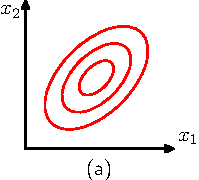
\includegraphics[width=.25\textwidth]{Figure28a.pdf}
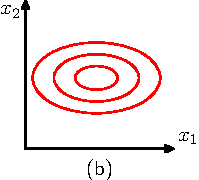
\includegraphics[width=.25\textwidth]{Figure28b.pdf}
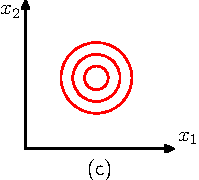
\includegraphics[width=.25\textwidth]{Figure28c.pdf}
\end{center}
~\\
\tiny Bishop PRML Figure 2.8
}

\frame[shrink=5]{\frametitle{A (super brief) primer on covariance matrices. (more details/intuition in second half of course?)} 
%\begin{columns}
%\begin{column}{4.5cm}

%\end{column}
\begin{center}
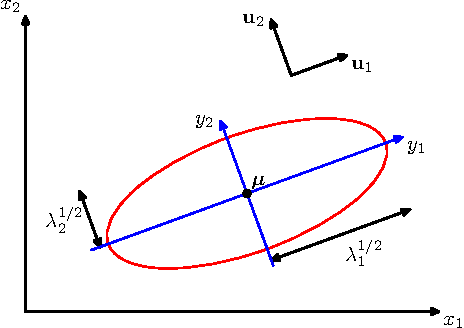
\includegraphics[width=.45\textwidth]{Figure27.pdf}
\\
\tiny Bishop PRML Figure 2.7
%\end{column}
\end{center}
%\begin{column}{8cm}
\begin{itemize}
\item \pause Covariance matrices are symmetric.
\item \pause Diagonal entries: variances along coordinate-axes
\item \pause Eigenvectors: principal axes of ellipsoid
\item Eigenvalues:  variances along eigen-vectors
\item Eigenvector with maximal/minimal eigen-value: Direction of maximal/minimal variance 
\item \pause Covariance matrices are `positive definite', i.e. all their eigenvalues are non-negative.
\item \pause Most of this can be derived from $a^\top \mbox{Cov}(X) a= \mbox{Var}(a^\top X)$
\end{itemize}
%\end{column}
%\end{columns}


}


\section{A generative model: Class-conditional Gaussians}
\frame{\frametitle{A tale of two Gaussian: We can use a probablistic model of the data for classification} 
\begin{center}
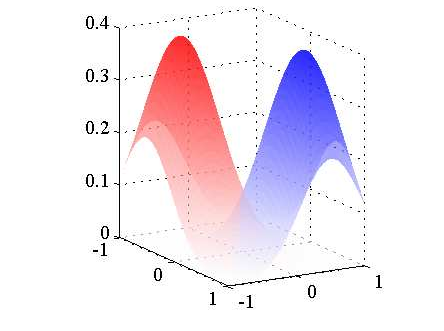
\includegraphics[width=.35\textwidth]{Figure410a.pdf}
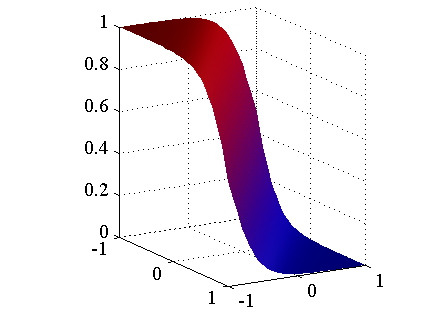
\includegraphics[width=.35\textwidth]{Figure410b.pdf}
\end{center}

\begin{itemize}
\item Suppose that each of the two classes is modelled by a Gaussian: $x | x \in C_+ \sim \mathcal{N}\left(\mu_+, \Sigma_+\right)$, $x | x \in C_- \sim \mathcal{N}\left(\mu_-, \Sigma_-\right)$, 
\item ~[On board] Calculation of posterior class probabilities and decision criterion
\item \pause If we assume $\Sigma_+=\Sigma_-$, we get $\omega_{gauss} \propto \Sigma_+^{-1} (\mathbf{m}_+-\mathbf{m}_-)$
\item Note: We take the $t_n$ as given and built a model of $x_n | t_n$, contrast with linear regression, where we took $x_n$ as given and modelled $t_n |x_n$.
\end{itemize}
\tiny Bishop PRML Figure 4.10
}

\frame{\frametitle{This approach directly generalizes to classification with unequal covariances and multi-class classification.}
\begin{center}
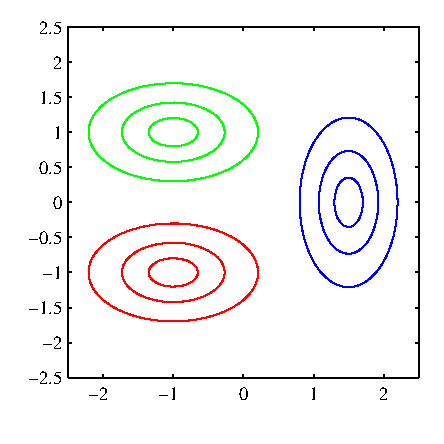
\includegraphics[width=.35\textwidth]{Figure411a.pdf}
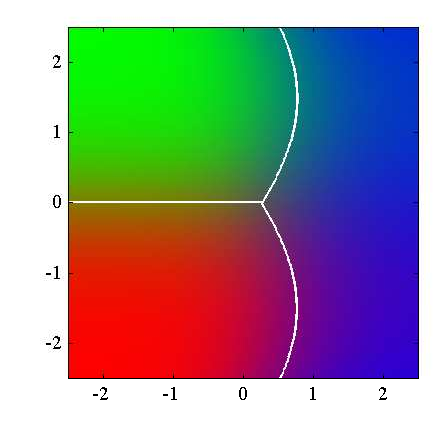
\includegraphics[width=.35\textwidth]{Figure411b.pdf}
\end{center}
\begin{itemize}
\item Quadratic discriminant analysis: $\Sigma_+ \neq \Sigma_o$, decisison boundary is of form $y(\xx) = \xx^\top A \xx+\omega^\top \xx +\omega_o$
\item Multi-class: Assign each data-point to class with highest posterior probability (or calculate best assignment from cost-function). 
\end{itemize}
\tiny Bishop PRML Figure 4.10
}

\frame{\frametitle{A simple nonlinear classifier can be constructed from kernel density estimates of the probability densities.}

\begin{columns}
\begin{column}{4cm}

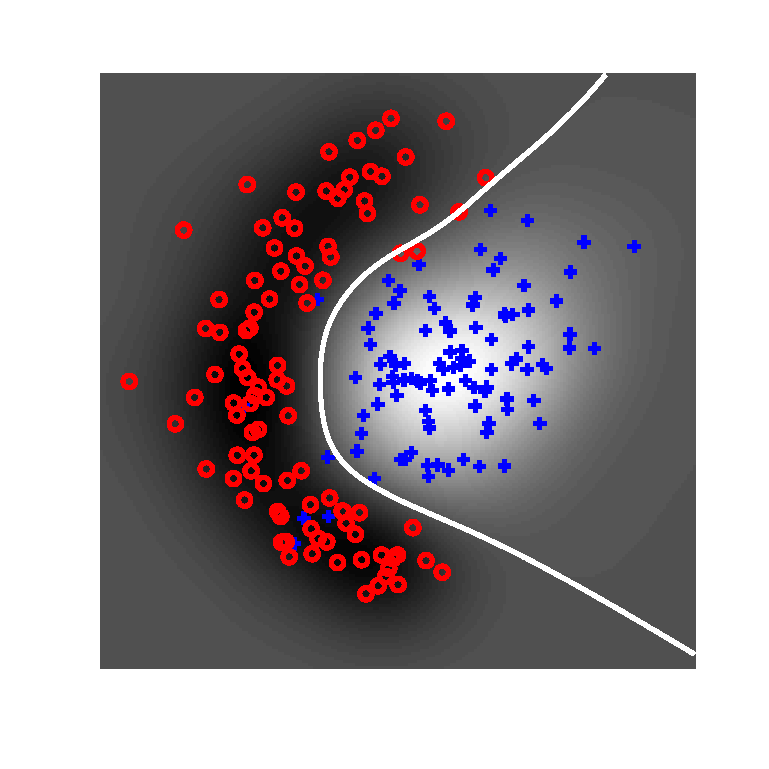
\includegraphics[width=\textwidth]{NonLinClassification.pdf}
\end{column}
\begin{column}{7cm}
\begin{itemize}
\item Idea: Once we have an estimate of the class-conditional densities $P(x| t=\pm 1)$, we can construct a rule from $d(x)=P(x| t=+ 1)-P(x| t=- 1)$.
\item \pause Use \alert{kernel density estimation} to estimate  $P(x| t=\pm 1)$, i.e. place a `Gaussian bump' on each data-point:
\begin{align}
P(x| t=1) =\frac{1}{Z}\sum_{n_+} \exp\left( \frac{x-x_n}{\sigma}\right)^2
\end{align}
\end{itemize}
\end{column}
\end{columns}
\pause
This leads to a classifier of the form
\begin{align}
d(x)= \sum_{n} \alpha  t_n \exp\left( \frac{x-x_n}{\sigma}\right)^2
\end{align}
\pause
\alert{Support vector machine with radial basis functions} has decision rule \begin{align}
d(x)=\sum_{n}  \alpha_n \exp\left( \frac{x-x_n}{\sigma}\right)^2
\end{align}
}




\frame{\frametitle{Summary: One for the price of three.} 
\begin{itemize}
\item Today, you learned about three different algorithms for binary classification with linear decision rules. 
\item \pause One was based on a hack, the second one on a plausible (but ad-hoc) criterion, and the third one an a probababilistic model of the data.
\item \pause All three algorithms are equivalent.
\item \pause We showed that the Fisher discriminant and the probabilistic model based on two Gaussians have the same  decision criterion. In fact, it can be shown that linear regression has the same weights (Bishop 4.1.5)
%\item \pause The moral: Great motivations are great, but the actual algorithm matters, and it is important to check connections with other algorithms.
\item The third motivation had immediate extensions to nonlinear algorithms and multi-class classification, and posterior probabilities.
\item \pause Next week, we will learn an algorithm which actually is different, and usually better than the ones discussed today.
\end{itemize}
}



\end{document}




	


\documentclass[10pt, handout]{beamer}
\setbeamertemplate{navigation symbols}{}
\usefonttheme{serif} 
\usepackage{amsmath}
\usepackage{amssymb}
\usepackage{graphicx}
\usepackage{cite}
\usepackage{color} 
\usepackage{setspace}
\usepackage{hyperref}

\newcommand{\xx}{{\bf{x}}}

\begin{document}
\title{Machine Learning I Lecture VII:\\ Logistic Regression}   
\author{Jakob H Macke\\ Max Planck Institute for Biological Cybernetics\\ Bernstein Center for Computational Neuroscience} 
\date{\today} 

\frame{\titlepage} 

%\frame{\frametitle{Today: Back to basics of probability theory}} 


\frame{\frametitle{Plan for today}\tableofcontents} 

\section{Logistic Regression}

\frame{\frametitle{For the linear classification model, we assumed the class-conditional distributions to be Gaussian}
\begin{itemize}
\item We assumed $x| (t=1) \sim \mathcal{N}(\mu_+, \Sigma_+)$ and $x| (t=-1) \sim \mathcal{N}(\mu_-, \Sigma_-)$, and two class-probabilities $P(t=1)$ and $P(t=-1)$.
\item \pause This is called an \alert{generative model}, as we have written down a full joint model over the data. 
\item \pause We saw that violations of the model assumption can lead to `bad' decision boundaries.
\end{itemize}
\begin{center}
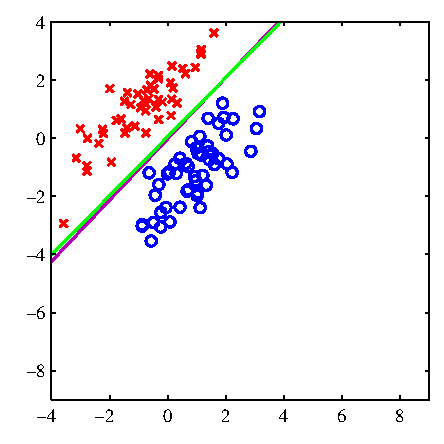
\includegraphics[width=.35\textwidth]{Figure44a.pdf}
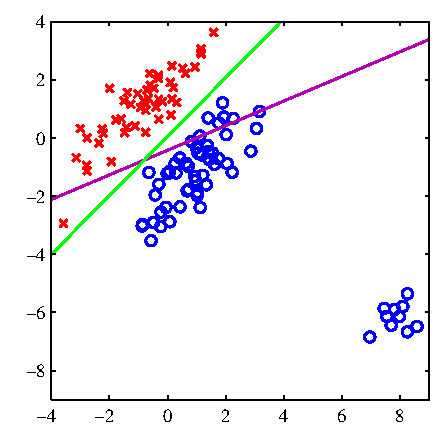
\includegraphics[width=.35\textwidth]{Figure44b.pdf}

\tiny Figures from Bishop PRML, 44a and b
\end{center}
} 

\frame{\frametitle{For regression, we assumed Gaussian outputs, but did not need assumptions about the distribution of inputs.}
\begin{itemize}
\item For linear regression, we conditioned on $x$, and assumed a Gaussian distribution over $t$: $t|x \sim \mathcal{N}(y(x), \gamma^2)$
\item \pause We maximized the conditional log-likelihood $L(\omega)=\sum_n \log p(t_n|x_n, \omega)$, i.e we assumed that the $x$ were given.
\item \pause Therefore, this approach to linear regression works for \alert{any} distribution over $x$.
\item $x$ is typically high-dimensional, so it is difficult to make appropriate distributional assumptions for it. 
\end{itemize}
\begin{center}
\includegraphics[width=.4\textwidth]{Figure128.pdf}

\tiny Figure Bishop PRLM 128
\end{center}
} 



\frame{\frametitle{We can define a discriminative model for classification by modelling the conditional class probabilities.}
\begin{itemize}
\item From the homework-exercise, we know that $P(t=1 | z(x))=\sigma(z(x))$ where $\sigma(z)=1/(1+\exp(-z))$ and $z(x)=
\omega^\top x+\omega_o$.
\item Notation is simpler if we use $0$ and $1$ as class labels, so we define $s_n=1$ as the label for the positive class, and $s_n=0$ als label for the negative class.
\item In other words, $s |x \sim \mbox{Bernoulli}(\sigma(y(x))$.
\item Also, we set $y_n=\sigma(z(x))$.
\item \pause The parameters of $z(x)=\omega^\top x+ \omega_o$ can be learned by maximizing the conditional log-likelihood $L(\omega)=\sum_n \log p(t_n|x_n, \omega)$ [on board]
\item \pause This is an \alert{discriminative} approach to classification, as we only model the labels, and not the inputs.
\item 
\pause Decision rule and function shape of $p(t|x)$ will be the same for the generative (`Linear Discriminant Analysis') and the discriminative model, but the parameters were obtained differently.
\end{itemize}
} 

\section{Maximum likelihood estimation of Logistic Regression}


\frame{\frametitle{Maximum likelihood estimation of Logistic Regression}
\begin{center}
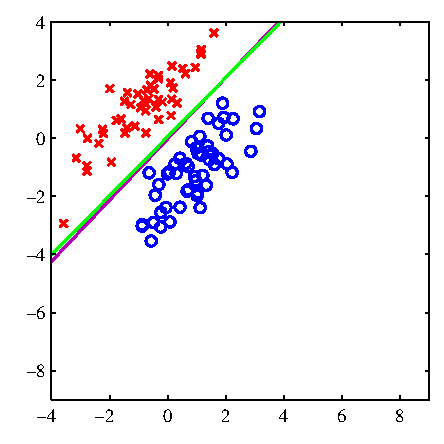
\includegraphics[width=.35\textwidth]{Figure44a.pdf}
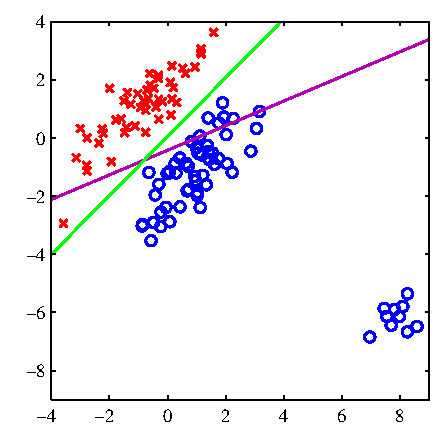
\includegraphics[width=.35\textwidth]{Figure44b.pdf}

\tiny Bishop PRML Figure 44 a and b
\end{center}
\begin{itemize}
\item This algorithm is called \alert{logistic regression}, and is a \emph{much} better algorithm than the algorithms we discussed last week.
\item Need to optimize log-likelihood numerically.
\item \pause People typically minimize the negative log-likelihood $\mathcal{L}$ rather than maximize the log-likelihood...
\item \pause To numerically minimize the negative log-likelihood, we need its gradient (and maybe its hessian) [on board]
\end{itemize}
}

\frame{\frametitle{The cost-function for logistic regression is convex.}
\begin{center}
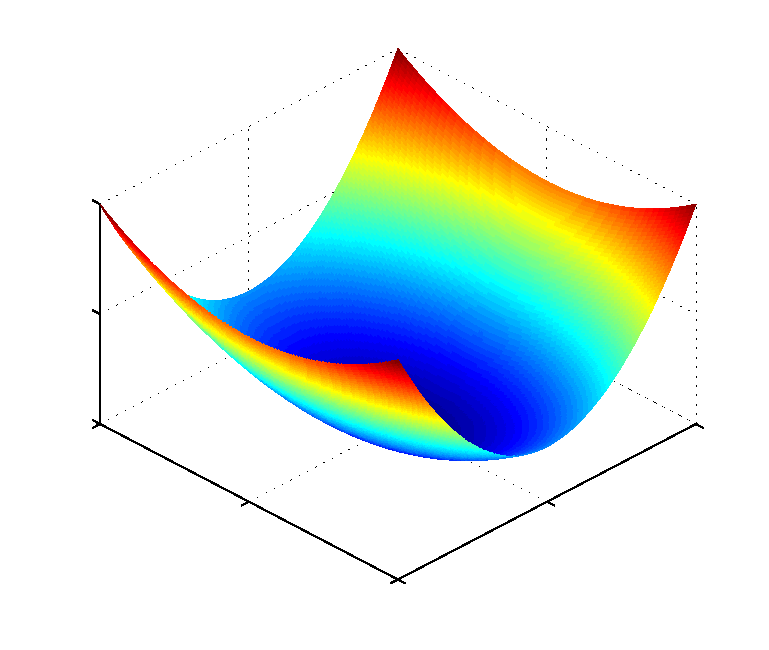
\includegraphics[width=.48\textwidth]{Convex.pdf}
\includegraphics[width=.48\textwidth]{NotConvex.pdf}
\end{center}
\begin{itemize}
\item \pause Fact: The negative log-likelihood is \emph{convex} -- this makes life much more easier. 
\item \pause There are no local minima to get stuck in, and there is good optimization techniques for convex problems. 
\end{itemize}
}




\frame{\frametitle{\emph{Gradient descent} is a simple method for numerically minimizing a function.}
\begin{itemize}
\item The gradient $\nabla \mathcal{L}$ of a function points into the direction of steepest descent.
\item \pause Gradient descent: 'run down the gradient' $\omega_{new}=\omega_{old}-\alpha \nabla \mathcal{L}_\omega$, with learning rate $\alpha$.
\item \pause Slightly more sophisticated version: numerically optimize $\alpha$ for each step by doing a \emph{line search}.
\item \pause Convergence can be very slow if cost-function has `valleys'.
\end{itemize}
\includegraphics[width=.7\textwidth]{BoydGradientDescent}

\tiny Figure from Stephen Boyd, Convex Optimization
}

\frame{\frametitle{\emph{Iterative Least Squares:} Approximate by parabola, minimze, iterate.}
\includegraphics[width=.8\textwidth]{Newton0}
}

\frame{\frametitle{\emph{Iterative Least Squares:} Approximate by parabola, minimze, iterate.}
\includegraphics[width=.8\textwidth]{Newton1}
}

\frame{\frametitle{\emph{Iterative Least Squares:} Approximate by parabola, minimze, iterate.}
\includegraphics[width=.8\textwidth]{Newton2}
}


\frame{\frametitle{\emph{Iterative Least Squares:} Approximate by parabola, minimze, iterate.}
\includegraphics[width=.8\textwidth]{Newton3}
}

\frame{\frametitle{\emph{Iterative Least Squares:} Approximate by parabola, minimze, iterate.}
\includegraphics[width=.8\textwidth]{Newton4}
}
\frame{\frametitle{\emph{Iterative Least Squares:} Approximate by parabola, minimze, iterate.}
\includegraphics[width=.8\textwidth]{Newton5}
}
\frame{\frametitle{\emph{Iterative Least Squares:} Approximate by parabola, minimze, iterate.}
\includegraphics[width=.8\textwidth]{Newton6}
}



\frame{\frametitle{\emph{Iterative Least Squares} is a more efficient method for minimizing the cost-function}
\begin{itemize}
\item Newton-Raphson: $\omega_{new}=\omega_{old}-\alpha (\nabla \nabla \mathcal{L})^{-1}\nabla L_\omega$ 
\item Pre-multiplying the gradient by the inverse-hessian speeds up convergence `along valleys' (analogy with LDA)
 \item Motivation: For quadratic functions $F(x)=a+b^\top x+ x^\top B x$, Newton-Raphson finds the minimum in one iteration.
 \item In this contex, Newton-Raphson (with $\alpha=1$) is often called \alert{iterative least squares}.
 \item Note: Newtwn's method can be bad if problem is not convex, and can be slow if it is difficult to calculate/invert the Hessian. A large number of optimization algorithms exist which do not require the (complete) Hessian (quasi Newton/BFGS, etc..). 
% \item Any (reasonable) optimization algorithm requires the gradient.
\end{itemize}
}

\frame{\frametitle{Visualizing the cost-function of logistic regression}

[on board]

}

\section{Bayesian Logistic Regression: Approximating the posterior distribution}
\frame{\frametitle{Bayesian inference for this model does not have a closed form solution}
\begin{itemize}
\item Typically use Gaussian prior on $\omega$.
\item For linear regression, posterior distribution was Gaussian, with closed-form solutions for the mean and covariance.
\item For logistic regression, the posterior distribution is non-Gaussian.
\item \pause Popular approximation: Approximate posterior by a Gaussian
\begin{align}
p(\omega|D) \approx \mathcal{N}(\mu_{post}, \Sigma_{post})
\end{align}
\item \pause Different methods exist for finding `good' $\mu_{post}$ and $\Sigma_{post}$: Expectation Propagation (EP), Laplace Approximation, Variational Inference
\end{itemize}

}

\frame{\frametitle{The Laplace-Approximation is a simple Gaussian approximation to the posterior}
\begin{itemize}
\item \alert{Laplace approximation:} $\mu_{post}=\omega_{MAP}$, $\Sigma_{post}=\left(\nabla \nabla_\omega L   \right)^{-1}$. 
\item Take MAP as mean, and inverse hessian at MAP as covariance.
\item \pause Motivation: Curvature matching, Taylor-expansion [on board]
\item \pause Q: When will the Laplace approximation fail?
\end{itemize}
\includegraphics[width=.49\textwidth]{Figure414a.pdf}
\includegraphics[width=.49\textwidth]{Figure414b.pdf}

\tiny Figure from Bishop PRML Figures 414a and b
}

\frame{\frametitle{The posterior distribution can be used to calculate the predictive distribution and to optimze hyper-parameters}
[on board]

}


%\section{LR's popular little brother-- support vector machines}

%\section{The exam}



\frame{\frametitle{One last bit of business: The exam}

\begin{itemize}
\item Next Friday, 2pm \emph{sharp}.
\item You will have 90 minutes.
\item You are allowed to use a pen or other writing utensils and your brain, no other tools/materials/books/notes will be allowed.
\item All mobiles phones need to be switched off.
\item Master-Students: Graded
\item Everyone else: Pass/Fail. If you want a grade for whatever reason, let me know (but it might not have any official meaning).
\end{itemize}
} 


\frame{\frametitle{This is the end.}

Have fun in the second half of the course!
\vspace{1cm}

\pause
If you did like (some bits) from these lectures ...


\vspace{1cm}
... and want to do a lab-rotation on using machine-learning methods to analyse neural data and to model neural population dynamics

\vspace{1cm}
... write an email to jakob\@tuebingen.mpg.de.

} 


\end{document}



	

\pagebreak
	
    \part{Unsupervised Learning}    
   	{\Large Lecturer: Prof. Dr. Bethge}\\[1cm]

\textbf{Examples of unsupervised learning applications}
\begin{itemize}
	\item \emph{density estimation} (e.g. texture synthesis), image compression
	\item level set estimation
	\item clustering/mode finding e.g. spike sorting; algorithm Mixture of Gaussians
	\item metric learning e.g. 3D visualization; algorithm multidimensional scaling
	\item feature extraction -> representation learning, e.g. whitening; algorithm principle component analysis
\end{itemize}

\section{Set algebras, measures, and probabilities}
\begin{itemize}
\item {\bf Overview for the mathematical construction of random variables}
\begin{itemize}
\item Sample Space $S$ (often also $\Omega $). $s\in S$ ``outcomes''
\item Boolean Algebra (or Sigma Algebra)  $\mathcal{B}(S)$ and $A \in \mathcal{B}(S)$ are called ``events''. An event $A$ is realized if an outcome $s$ is in $A$. \\For example, $\mathcal{B}(S)=\mathcal{P}(S)$
\item Measure $m: \mathcal{B}(S) \to [0,\infty)$ and $m(A\dot\cup B) = m(A) + m(B)$
\item probability measure $p(S)=1$, if $m$ is a measure with $m(S)<\infty$ then $p(A) := m(A)/m(S)$ is a probability measure.
\item random variables: consider $M \in \mathcal{B}(S)$ with $M=\{s \in S: X(s) < \vartheta\} \subseteq S$
\end{itemize}

\item {\bf Power Set:}  $\mathcal{P}(S) := \{A\subseteq S\}$, $|\mathcal{P}(S) |= 2^{|S|}$

\item {\bf Boolean Algebra:}  $\mathcal{B}(S) \subseteq \mathcal{P}(S)$ is called a {\it Boolean Algebra} iff
\begin{itemize}
\item[(i)] $A \in \mathcal{B}(S)  \Rightarrow \overline{A} \in \mathcal{B}(S)  $
\item[(ii)] $A, B \in \mathcal{B}(S)  \Rightarrow A \cup B \in \mathcal{B}(S)  $ 
\end{itemize}
Examples:
\begin{itemize}
\item[(i)] $\{ \emptyset, S\}  $ and $\mathcal{P}(S)$ are Boolean Algebras.
\item[(ii)] If $a\in S$ then $\{\emptyset, \{a\}, S-\{a\}, S\}$ is the Boolean Algebra {\it generated by} $a$.
\item[(iii)] $I(R)$ is defined to be the smallest Boolean Algebra which contains all open intervals $(a,b)$ for which $-\infty \le a < b\le \infty$. 
\end{itemize}

\item {\bf Sigma-Algebra:}  $\mathcal{B}(S) \subseteq \mathcal{P}(S)$ is called a Sigma-Algebra if  
\begin{itemize}
\item[(i)] $A \in \mathcal{B}(S)  \Rightarrow \overline{A} \in \mathcal{B}(S)  $
\item[(ii)] For all sequences $A_1, A_2, \dots \in \mathcal{B}(S)  \Rightarrow \bigcup_{k=1}^\infty A_k \in \mathcal{B}(S)  $ 
\end{itemize}

\item {\bf Venn diagram} 

\end{itemize}

%\item {\bf Proposition 1 (Boolean laws):} 
\begin{proposition}[Boolean laws]
\begin{itemize}
\item[(B1)] Idempotency: $A \cup A = A$;   \hspace{.5cm} $A \cap A = A$
\item[(B2)] Associativity: $A \cap (B\cap C) = (A\cap B) \cap C$  
\item[(B3)] Commutativity: $A \cup B = B \cup A$;    \hspace{.5cm}  $A \cap B = B \cap A$
\item[(B4)] Distributivity: $A \cap (B\cup C)  = (A \cap B) \cup (A \cap C)$; \hspace{.5cm}  $A \cup (B\cap C)  = (A \cup B) \cap (A \cup C)$
\item[(B5)] de Morgan's law:  $\overline{A \cup B} = \overline{A} \cap \overline{B} $;    \hspace{.5cm}  $\overline{A \cap B} = \overline{A} \cup \overline{B} $
\item[(B6)] Complements: $ \overline{ \overline{A}} =  A$; \hspace{.5cm}  $A \cap \overline{A} = \emptyset$; \hspace{.5cm}  $A \cup \overline{A} = S$
\item[(B7)] Properties of $S$ and $ \emptyset$: \hspace{.2cm} $A \cup S = S$; \hspace{.5cm} $A \cup \emptyset = A$; \hspace{.5cm} $A \cap S = A$; \hspace{.5cm} $A \cap \emptyset = \emptyset$

\end{itemize}
\end{proposition}

\begin{itemize}

\item {\bf (Finite) Measure:} A mapping $m: \mathcal{B}(S) \rightarrow [0, \infty), A\in  \mathcal{B}(S) \to m(A) \in [0, \infty)$ is called a {\it measure} if for all $A,B \in \mathcal{B}(S)$ with $A\cap B = \emptyset$ holds: $m(A\cup B) = m(A) + m(B)$.\\(This property can be written compactly as $m(A\dot\cup B) = m(A) + m(B)$)

Examples:
\begin{itemize}
\item[(i)] $m(A) := |A|$ is the {\it counting measure}.
\item[(ii)] For $S=[a,b]$ and $\mathcal{B}(S)=\mathcal{I}([a,b])$ with $|a|, |b| < \infty$ the {\it Lebesgue Measure} is defined as $m([c, d]) := d-c$.
\item[(iii)] If $f(x) \ge 0$ for all $a \le x \le b$ with $\int_a^b f(x) dx <\infty$ then $m([c, d]) := \int_c^d f(x) dx $ is a measure.
\item[(iv)] For $S=R$ and $\mathcal{B}(S)=\mathcal{I}(R)$ the {\it Dirac Ma\ss} is given by $\delta_a(J) = 1$ if $a\in J$ and $\delta_a(J) = 0$ otherwise.
\end{itemize}

\item {\bf Proposition 2:} 
\begin{itemize}
\item[(i)] If $B\subseteq A$ then $m(A-B) = m(A) - m(B)$.
\item[(ii)] If $B\subseteq A$ then $m(B) \le m(A)$.
\item[(iii)] $m(\emptyset) =0$.
\item[(iv)] $m(A \cup B) = m(A) + m(B) - m(A\cap B)$.
\end{itemize}

\item {\bf Proposition 3:}\\
If $A,B \in \mathcal{B}(S)$ then:
\begin{itemize}
\item[(i)] $ (A \cap B) \in \mathcal{B}(S)$ since $ (A \cap B) = \overline{\overline{A} \cup \overline{B}}$.
\item[(ii)] $\emptyset, S$ belong to every Boolean Algebra, since for $A \in \mathcal{B}(S)$ also $\overline{A} \in \mathcal{B}(S)$ and $A \cap \overline{A} = \emptyset$ and $A\cup \overline{A} = S$ .
\item[(iii)] $\mathcal{B}_B(S) := B \cap \mathcal{B}(S) = \{A \cap B: A \in \mathcal{B}(S)\}$ is a Boolean Algebra if $B\ne \emptyset$.
\item[(iv)] $\mathcal{B}_B(S) \subseteq \mathcal{B}(S)$. 
\end{itemize}


\item {\bf Probability measure:} For a sample space $S$ and a Sigma Algebra $\mathcal{B}(S)$ a measure \, $P$ is a {\it probability measure} if $P(S)=1$.

\item {\bf Probability space:} A probability space consists of the triple $(S,\mathcal{B}(S), P)$ where $S$ is the sample space, $\mathcal{B}(S)$ the event algebra (which is a Boolean or a sigma algebra) and $P$ is a  probability measure on $\mathcal{B}(S)$. 

\item {\bf Proposition 4:} 
\begin{itemize}
\item[(i)] $0 \le P(A) \le 1$.
\item[(ii)] $P(\overline{A}) = 1-P(A)$.
\item[(iii)] If $\mathcal{E}= \{E_1, E_2, \dots, E_n\}$ is a partition of $S$ (that is $S= \bigcup_{k=1}^n E_k$ and $E_l \cap E_m = \emptyset$), then \quad $\sum_{k=1}^n P(E_k) = 1$ \quad and \quad $P(A)=\sum_{k=1}^n P(A\cap E_k)$.
\end{itemize}

\item {\bf Specification of probabilities}
\begin{itemize}
\item[(i)] As a limiting value of relative frequencies: $P(A) = \lim_{n\to \infty} \frac{r_n(A)}{n}$
\item[(ii)] Symmetrie assumptions (e.g. if we assume $P(s)=P(s^\prime)$ for all $s,s^\prime \in S$ then it follows: $P(s) = 1/|S|$).
\item[(iii)] Subjective probabilities (based on Cox axioms) can be determined via betting games.
\end{itemize}
\item {\bf Conditional probabilities:}
If $(S,\mathcal{B}(S), P)$ is a probability space and $B \in \mathcal{B}(S)$ then the restriction of $P$ to the reduced Sigma-Algebra $\mathcal{B}_B(S):=\{B\cap A: A \in \mathcal{B}(S)\}$ defines a measure \ $M_B: \mathcal{B}_B \to [0,\infty)$. If in addition $P(B) >0$, then $P_B: \mathcal{B}_B(S) \to [0,1], \quad A_B \mapsto P_B(A_B) :=  M_B(A_B)/P(B)=P(A_B)/P(B), \, \forall A_B \in \mathcal{B}_B(S)$ is a probability measure on $\mathcal{B}_B(S)$.\\
The $A_B\in \mathcal{B}_B(S)$ usually originate from intersection of the elements of the original Sigma-Algebra $\mathcal{B}(S)$ with the event $B$.
\item {\bf Independence:}\\
Two events $A$ and $B$ are {\it statistically independent} iff $P(A\cap B) = P(A) P(B)$.
\item {\bf Proposition 5:} 
\begin{itemize}
\item[(i)] Two events $A$ and $B$ are (statistically) independent if $P(A)=0$ or $P(B)=0$.
\item[(ii)] If two events $A$ and $B$ are independent and $P(A)>0$, then: $P(B|A)=P_A(B)=P(B)$.
\item[(iii)] If two events $A$ and $B$ are independent and $P(A)>0$, then $A$ and $\overline{B}$ are independent as well.
\end{itemize}

\end{itemize}

\section{Random Variables}
\begin{itemize}
\item {\bf Cumulative distribution function (cdf):} 
Any univariate random variable can be uniquely defined by the cumulative distribution function:
$$
F(x) = P(\{s \in S: X(s) \le x\}), \quad \forall x \in S^\prime
$$
It holds:
\begin{itemize}
\item[(i)] $F$ is a nondecreasing function.
\item[(ii)] $\lim_{x\to -\infty} F(x)= 0$, $\lim_{x\to \infty} F(x)= 1$
\item[(iii)] Any function that fulfills (i)+(ii) is a cdf.
\item[(iv)] $ P(\{s \in S: X(s) > x\}) = 1-F(x)$
\item[(v)] $ P(\{s \in S: x_1 < X(s) \le x_2\}) = F(x_2)-F(x_1)$
\item[(vi)] discrete case: probability mass function / point probability $p(x) = F(x) - \lim_{\epsilon \to 0}F(x-\epsilon)$
\item[(vii)] continuous case: probability density function (pdf) $\rho(x) = \frac{d}{dx} \mathcal{F}(x)$
\end{itemize}


\item {\bf Expectation (value):} 
$$
E[X] = \sum_{k=1}^n p(x_k) x_k , \quad E[f(X)] = \sum_{k=1}^n p(x_k) f(x_k) 
$$
\item {\bf Moments:} 
$$
E[X^m] =  \sum_{k=1}^n p(x_k) x_k^m
$$
\item {\bf Variance:} 
$$
Var[X]= E[X^2]-E[X]^2
$$

\end{itemize}
\vfil 



   	\begin{center}
{\LARGE\bf  
Machine Learning WS2012/13 (Unsupervised Learning)}\\[.5cm]
{\Large Lecturer: Prof. Dr. Bethge\\[1cm]

\bf 2. Multivariate Distributions
}
\end{center}


\begin{itemize}

\item {\bf Joint distribution:} 
$$
p(x_i, y_j) = P(\{s \in S: X(s) = x_i\} \cap \{s \in S: Y(s) = y_j\})
$$

The following properties hold:
\begin{itemize}
\item[(i)] $\sum_i p(x_i, y_j) = p(y_j)$
\item[(ii)]  $\sum_j p(x_i, y_j) = p(x_i)$
\item[(iii)]  $\sum_i \sum_j p(x_i, y_j) = 1$\\
\end{itemize}

\item {\bf Joint cumulative distribution function:} 
$$
F(x) = P(\{s \in S: X(s) \le x\} \cap \{s \in S: Y(s) \le y\}), \quad \forall (x,y) \in (S_x \times S_y)
$$
The following properties hold:
\begin{itemize}
\item[(i)] $F(x_{k+1},y) - F(x_k,y) = p(x_{k+1},y)$,   \quad $F(x,y_{k+1}) - F(x,y_k) = p(x,y_{k+1})$
\item[(ii)] $F$ is a nondecreasing function in $x$ and $y$.
\item[(iii)] $\lim_{x\to -\infty} \lim_{y\to -\infty}  F(x,y)= 0$, \quad $\lim_{x\to \infty} \lim_{y\to \infty}  F(x,y)= 1$
\item[(iv)] $ P(\{s \in S: X(s) > x\} \cap \{s \in S: Y(s) \le y\})) = F(\infty,y)-F(x,y)$, \\ $ P(\{s \in S: X(s) > x\} \cap \{s \in S: Y(s) > y\})) = 1-F(\infty,y)-F(x,\infty)+F(x,y)$
\item[(v)] $ P(\{s \in S: x_1 < X(s) \le x_2\} \cap \{s \in S: y_1 < Y(s) \le y_2\}) = F(x_2,y_2) - F(x_2,y_1)-F(x_1,y_2) + F(x_1,y_1)$
\end{itemize}

\item {\bf Covariance:} 
$$
Cov[X,Y]= E[XY]-E[X]E[Y], 
$$
\item {\bf Covariance matrix:} for  $n$ random variables $X_1, \dots , X_n$ the {\it Covariance matrix} is defined by:
$$
 C_{ij} := Cov[X_i, X_j] = E[X_i X_j] - E[X_i] E[X_j]
$$
\item {\bf Independence:} 
Two random variables $X,Y$ are {\it (statistically) independent} if their joint distribution is factorial: $p(x,y)= p(x) p(y)$ or, equivalently, if their joint cdf is factorial: $F(x,y)=F(x)F(y)$
\item {\bf Proposition 1:} 
\begin{itemize}
\item[(i)] The expectation value is a linear form: $E[aX +bY+c]= a E[X]+bE[Y]+c$
\item[(ii)] $Var[X] = Cov[X,X]$
\item[(iii)] $Cov[X, Y] = E[(X - E[X])(Y-E[Y])]$ \,\, and hence \,\, $Var[X] = E[(X - E[X])^2]$
\item[(iv)] The covariance is a bilinear form $Cov[aX+b, cY+d]=ac \, Cov[X, Y] $ \,\, and hence \,\, $Var[aX] = a^2\, Var[X]$
\item[(v)] If  $X,Y$ independent, then $Cov[X,Y] = 0$
\item[(vi)] The inversion is not warranted. Counter example: $p(x,y) = 1/8$ for all integers $x,y$ for which $|x| + |y| =2 $ and zero otherwise. Then\,\,  $Cov[X,Y] = 0$ \,\, but\,\, $p(x,y)\ne p(x) p(y)$.
\item[(vii)] $Var[X+Y] =  Var[X] + Var[Y] + 2 Cov[X,Y]$ or more generally:\\[.2cm] $Var\left[\sum_{k=1}^n X_k \right] = \sum_{k=1}^n \sum_{j=1}^n Cov[X_k, X_j] = \sum_{k=1}^n Var[X_k] + \sum_{j\ne k} Cov[X_k, X_j] $
\item[(viii)] $(Cov[X, Y])^2\le Var[X] \, Var[Y]$ \\(Hint: Let $\tilde X:=X-E[X]$, $\tilde Y:=Y-E[Y]$, and $Z:= (\tilde X-t\tilde Y)^2$. Then $E[Z]=t^2 E[\tilde Y^2]-2tE[\tilde X\tilde Y]+E[\tilde X^2] \ge 0 \forall t$ and hence $E[\tilde X\tilde Y]^2 \le E[\tilde X^2]E[\tilde Y^2]$ because $at^2 + bt+c \ge 0\,\, \forall t \,\, \Leftrightarrow \,\, b^2\le 4ac$.) 
\item[(ix)] The covariance matrix is positive semi-definite: $C=AA^\top=UDU^\top$ mit $UU^\top=U^\top U=I$ (i.e. U is orthogonal) and $D_{ij}=Var[X_i] \, \delta_{ij} \ge 0$ (i.e. non-negative eigenvalues).
\item[(x)] Decomposition of {\it total variance}: $Var[X] = E[Var[X|Y]] + Var[E[X|Y]]$
\end{itemize} 
\item {\bf IID Random variables:} $X_1, \dots, X_n$ are called ``{\it independent, identically distributed (i.i.d.)}'', iff $p(x_1, \dots, x_n)=\prod_{k=1}^n p_k(x_k)$  \,\, and \,\, $p_1(x)=p_2(x)=\dots = p_n(x)= p(x)$.
\item {\bf Random Walk:} A sequence of random variables $\{S_n\}$ with $S_n=\sum_{k=1}^n X_k$ is called a ``{\it Random Walk}'', iff $X_1, \dots, X_n$ are 
i.i.d. random variables. Computing the expectation or the variance of $\{S_n\}$ generates a sequence $\{\mu_n\}$ or $\{\sigma^2_n\}$, respectively, with
$$
\mu_n=:E[S_n]=nE[X_1]
$$ 
$$
\sigma^2_n=:Var[S_n]=nVar[X_1]
$$ 
\item {\bf Binomial distribution:} A {\it binomial} random variable $k$ has the following distribution:
$$
p(k) = {n \choose k} \lambda^k (1-\lambda)^{n-k}, \quad 1\le k \le n 
$$
It describes the distribution of the $n$-th element of a random walk where $k=S_n$ is the sum over $n$ i.i.d. Bernoulli random variables $X \in \{0,1\}$. Thus, it holds:
$$
E[k] = n\, \lambda, \quad Var[k]= n \, \lambda (1-\lambda)
$$
\item {\bf Multinomial distribution:} A {\it multinomial} random variable is a multivariate random variable $\mathbf{k}$ and has the following distribution:
$$
p(\mathbf{k}) = \frac{n!}{k_1! \cdot \dots \cdot k_m!} \,\, \lambda_1^{k_1} \cdot \dots \cdot \lambda_m^{k_m}, \quad \sum_{j=1}^m k_j = n 
$$
It describes the distribution of the sum over $n$ i.i.d. categorical random variables $\mathbf{X} \in \{\mathbf{e}_1, \dots, \mathbf{e}_m\}$ with $\mathbf{e}_k$ being the standard basis vector whose $k$-th component is one and all other components are zero. It holds:
$$
E[k_j] = n\, \lambda_j, \quad Var[k_j]= n \, \lambda_j (1-\lambda_j), \quad Cov[k_i, k_j]= -n \, \lambda_i \,\lambda_j 
$$
\item {\bf Poisson distribution:} A {\it Poisson} random variable $k$ has the following distribution:
$$
p(k) = \frac{\mu^k}{k!} e^{-\mu}, \quad 0\le k \le n
$$
It is obtained as a limiting case for $n \to \infty$ subject to $E[k]=n\lambda=\mu$. It holds:
$$
E[k] = Var[k]= \mu
$$
\item {\bf Geometric Distribution:} A {\it geometric random variable} $k$ has a {\it ``discrete exponential''} distribution:
$$
p(k) = (1-\lambda)^{k-1} \lambda = (e^{\tilde \lambda}-1) \, e^{-\tilde \lambda \, k}, \quad  k \ge 1, \quad \mbox{with } \tilde \lambda = -\log(1-\lambda) \ge 0
$$
For example it is obtained, when asking for the probability that the waiting time to observe a $1$ only after $k$ Bernoulli experiments with parameter $\lambda$. It holds
$$
E[k] = \frac{1}{\lambda}, \quad Var[k]= \frac{1-\lambda}{\lambda^2}
$$
\item {\bf Boltzmann distribution:} For any function $E(\mathbf{x})$ the Boltzmann distribution is defined by
$$
p(\mathbf{x}) = \frac{1}{Z} \exp(-\beta E(\mathbf{x})) 
$$
where $E$ is called the {\it energy} and $Z=\sum \exp(-\beta E(\mathbf{x}))$ (in the discrete case) or  $Z=\int \exp(-\beta E(\mathbf{x})) d\mathbf{x}$ (in the continuous case) is called the {\it partition function}. The distribution is obtained by maximizing the entropy under the constraint of a fixed mean $E[\mathbf{x}] = E_0$.

\item {\bf Normal distribution:} A multivariate normal distributed random variable can be derived as the maximum entropy distribution for given mean $\mu$ and covariance $C$. It has the following density:
$$
\rho(\mathbf{x}) = \frac{1}{\sqrt{(2\pi)^n |C|}} \exp\left( -\frac{1}{2} (\mathbf{x-\mu})^\top C^{-1} (\mathbf{x-\mu}) \right)
$$
where $C=E[\mathbf{xx}^\top]- E[\mathbf{x}] E[\mathbf{x}^\top]$ is the covariance matrix. 

The {\it marginal distribution} $\rho(x_1, \dots, x_m)$ is given by
$$
\rho(\mathbf{x}) = \frac{1}{\sqrt{(2\pi)^n |C_m|}} \exp\left( -\frac{1}{2} (\mathbf{x-\mu_m})^\top C_m^{-1} (\mathbf{x-\mu_m}) \right)
$$
where $C_m = P_mCP_m^\top$ and $\mu_m = P_m \mu$ with $P_m=[e_1, \dots, e_m]$.

The {\it conditional distribution} $\rho(x_1, \dots, x_m| x_{m+1}, \dots, x_n)$ is given by
$$
\rho(x_1, \dots, x_m| x_{m+1}, \dots, x_n) = \frac{1}{\sqrt{(2\pi)^n |\tilde C|}} \exp\left( -\frac{1}{2} (\mathbf{x-\tilde \mu})^\top \tilde C^{-1}(\mathbf{x-\tilde \mu}) \right)
$$
where
$$
\tilde \mu = \mu({x_{m+1}, \dots, x_n})= C_{x_1, \dots, x_m| x_{m+1}, \dots, x_n} C_{x_{m+1}, \dots, x_n}^{-1} (x_1, \dots, x_m)^\top
$$
$$
\tilde C = C_m - C_{x_1, \dots, x_m| x_{m+1}, \dots, x_n} C_{x_{m+1}, \dots, x_n}^{-1} C_{x_1, \dots, x_m| x_{m+1}, \dots, x_n}^\top
$$

\item {\bf Elliptically contoured distribution:} An important generalization of the multivariate normal distribution is the class of elliptically contoured distributions for which the density takes the following simple form:
$$
\rho(\mathbf{x}) = f(||W\mathbf{x}||) .
$$

\end{itemize}


\vfil 


%%%%%%%%%%%%%%%%%%%%%%%%%%%%%%%%%%%%%%%%%%%%%%%%%%%%%%%%%%%%%%%%%%%%%%%
% \begin{wrapfigure}{r}{.28\textwidth} 
% \hspace{-.3cm}
% \fbox{
%% \includegraphics[height=0.45\textwidth]{./popRF4.pdf}
%% \includegraphics[height=0.45\textwidth]{./impulse_response4.pdf}
%}
%\vspace{-1cm}
%\end{wrapfigure}
%
%
%\item {\bf Elementar-Partition:} Sei $\mathcal{E}_0 \subset \mathcal{B}(S)$ definiert durch  $\mathcal{E}_0 := \{ \{s_k\} : s_k\in S\}$. Dann gilt:
%\begin{itemize}
%\item[(E1)] $\mathcal{E}_0$ ist eine Partition von $S$.
%\item[(E2)] $\mathcal{E}_0$ ist keine Boolsche Algebra. 
%\item[(E3)] Falls $m$ ein Ma\ss \ ist auf $\mathcal{B}(S)$ dann ist das Ma\ss \ eindeutig festgelegt, durch die Werte des Ma\ss es $m_k$  f\"ur die Elementar-Ereignisse $\{s_k\} \in \mathcal{E}_0$, also durch die Spezifikation: $m(\{s_k\})= m_k$.
%\item[(E4)] Insbesondere gilt f\"ur ein beliebiges Ereignis $A \in \mathcal{B}(S)$:
%$$
%m(A)=\sum_{ \{s_k\} \in \mathcal{E}_0} m(A \cap \{s_k\}) = \sum_{\{k\,:\, \{s_k\} \in (A \cap \mathcal{E}_0)\}} m_k
%$$
%\end{itemize}
%
%\item {\bf Zufallsvariable:} Eine Zufallsvariable $X$ ist eine (me\ss bare) Funktion von einem Wahrscheinlichkeitsraum $(S, \mathcal{B}(S), P)$ in einen Me\ss raum $(S^\prime,  \mathcal{B}(S^\prime))$. Die durch $X$ vorgegebene Abbildung induziert ein eindeutiges Wahrscheinlichkeitsma\ss \ auf $S^\prime$, welches durch die {\bf Wahrscheinlichkeitsverteilung} festgelegt ist. F\"ur {\it diskrete} Zufallsvariablen ist die Wahrscheinlichkeitsverteilung gegeben durch:
%$$
%p(x_j):= P(\{s \in S: X(s) = x_j\}), \quad \forall x_j \in S^\prime
%$$
%{\it Anmerkungen: }
%\begin{itemize}
%\item[(i)] F\"ur uns wird $S^\prime$ immer die Menge der reellen Zahlen sein. 
%\item[(ii)] F\"ur diskrete Zufallsvariablen k\"onnen wir immer die Potenzmenge als Ereignisraum w\"ahlen, d.h. $\mathcal{B}(S) = \{A : A\subseteq S\}$. In dem Fall ist jede Funktion von  $(S, \mathcal{B}(S), P)$ nach $(S^\prime,  \mathcal{B}(S^\prime))$ me\ss bar und somit eine Zufallsvariable.
%\end{itemize}
%
%Beispiele:
%\begin{itemize}
%\item[(i)] Sei $S=\{$``Kopf'', ``Zahl''$\}$ und $X($``Kopf''$)=1$ und $X($``Zahl''$)=0$. Dann ist $X$ eine (bin\"are) Zufallsvariable.
%\item[(ii)] Sei $S=\{1,2,3,4,5,6\}$ und $X(s)=1$ falls $s\in S$ ungerade und $X(s)=0$ falls $s\in S$ gerade. Dann ist $X$ eine (bin\"are) Zufallsvariable.
%\item[(iii)] Die Abbildung $f: \mathcal{B}(S) \to R$ mit $f(\{1,3,5\})=1$ und $f(\{2,4,6\})=0$ ist keine Zufallsvariable.
%\end{itemize}
%
%\item {\bf Praktischer Umgang mit diskreten Zufallsvariablen:} Man \"uberlegt sich, die Menge aller Elementar-Ereignisse, definiert eine Numerierung und eine Wahrscheinlichkeitsverteilung. Die Wahrscheinlichkeitsverteilung wird oft mit Hilfe eines {\bf Histograms} visualisiert, wo man die Werte der Wahrscheinlichkeitsverteilung als Funktion der Nummerierung auftr\"agt.\\[.2cm]
%{\it Beispiel:} Bei einer {\bf gleichverteilten Zufallsvariable} haben alle $n$ Elementarereignisse die gleiche Wahrscheinlichkeit: $p(1) = p(2) = \dots p(n) = 1/n$. Die Gleichverteilung spielt eine gro\ss e Rolle, da man h\"aufig aus Symmetrie-Annahmen heraus, sinnvoll ist allen Elementarereignissen die gleiche Wahrscheinlichkeit zu geben. In der statistischen Physik ist dies f\"ur das ``Mikrokanonische Ensemble'' der Fall, wo alle zul\"assigen Zust\"ande (diejenigen, die die vorgegebene Gesamtenergie haben) als gleichwahrscheinlich angenommen werden, da es keine weiteren Eigenschaften (wie zB Energie-Fluktuationen, Teilchenzahl-Fluktuationen, etc) gibt, die eine Symmetriebrechung nahelegen.
%
%\item {\bf Negative Binomialverteilung:} Eine {\it negativ-binomialverteilte} Zufallsvariable $k$ hat folgende WKT-Verteilung:
%$$
%p(n) = {n-1 \choose k-1} \lambda^k (1-\lambda)^{n-k}, \quad 1\le k \le n 
%$$
%Sie ist eine Verallgemeinerung der Wartezeit-Verteilung, wenn man nach der Anzahl der Experimente fragt, die man braucht um $k$ Einsen zu beobachten. Es gilt:
%$$
%E[k] = \frac{k}{\lambda}, \quad 
%$$
%\item {\bf Hypergeometrische Verteilung:} Eine {\it hypergeometrische} Zufallsvariable $k$ hat folgende WKT-Verteilung:
%$$
%p(k) = \frac{{s \choose k} {n-s \choose r-k}}{ {n \choose r}}  = \frac{{r \choose k} {n-r \choose s-k}}{ {n \choose s}} , \quad \max(0, r+s-n) \le k \le \min(r,s)
%$$

   	\section{Generative models}
In unsupervised learning we want to find generative models which allow us to generate new data
from previously made observations. We sometimes assume that observations are generated from a 
process which is not immediately observable from the data at hand. A general form of such a 
generative model can be written as:
\begin{align}
	\mb{x} = f(\mb{s})
	\label{eq:GM}
\end{align}
where $\mb{x}$ is a $D \times 1$ vector for a given observation, which is assumed to be 
generated by an arbitrary function $f(\mb{s})$. $\mb{s}$ is a $M \times 1$ vector of
source signals for the given observation. If $\mb{s}$ is known the problem of inferring
function $f(\mb{s})$ becomes a supervised learning task. However, if the sources are 
unknown the problem becomes an unsupervised learning task. UNder certain assumptions
it possible to infer sources from observations, this is called blind source separation.

\subsection{The linear generative model (LGM)} 
In the following we will only consider linear generative models for which equation \eqref{eq:GM}
takes the form:
\begin{align}
	\mb{x} = \mb{A s}
	\label{eq:LGM}
\end{align}
where $\mb{x}$ is an $D \times 1$ observation vector, $\mb{s}$ is the $M \times 1$ vector
of sources and $\mb{A}$ is a $D \times M$ transformation matrix. 
We distinguish three classes of LGM dependent on the dimensionality of $\mb{A}$:

\begin{enumerate}
	\item Overcomplete LGM: \textbf{A} is a fat matrix with $D<M$. \\
		  The number of source signals is assumed to be bigger than the dimensionality 
		  of our observations. The generative model is overcomplete since blow up the number
		  of possible sources.
	\item Undercomplete LGM: \textbf{A} is a flat matrix with $D>M$. \\
	      The undercomplete case is the inverse case an overcomplete LGM where the observations
	      are assumed to be generated from less sources that the dimensionality of our observations.
	\item Complete LGM: \textbf{A} is a square matrix with $D=M$, full rank 
	      and $\forall m = 1,\dots,M: \, \mathrm{Var}[\mb{s_m}] > 0.$ \\
	      In the complete case the number of source signals is assumed to equal the dimensionality
	      of our observations. In the following we will focus on complete LGMs.    
\end{enumerate}

% Table of UL algorithms used for different types of LGM
\begin{figure}[h]
\centering
\begin{tabular}{|l|l|}
\hline 
Generative Model & Unsupervised Learning algorithm \\ 
\hline 
Complete LGM & Principle Component Analysis (PCA), \\ 
             & Independent Components Analysis (ICA) \\ 
%\hline 
Overcomplete LGM & Factor Analysis, Independent Factor Analysis \\ 
\hline 
\end{tabular} 
\caption{Some examples of unsupervised leanring algorithms for the different classes of LGM. 
For all those algorithms it is assumed that observations \textbf{X} can be decomposed into 
sources $\mb{S}$ and transformation matrix $\mb{A}$.}
\end{figure}

\subsection{The complete LGM}
In this section we assume that our observations and signals have the same dimensionality,
i.e. we are dealing with a complete LGM. We further assume that matrix $\mb{A}$ is orthogonal
which means that:
\begin{align}
	 \mb{A}\TT \mb{A} = \mb{A} \mb{A}\TT = \imat_D
\end{align}
\noindent
We will further focus on normally distributed source signals as this will be relevant for the
orthogonality assumption with the application of principle component analysis. In fact orthogonality
of $\mb{A}$ is only guaranteed if our observations are normally distributed. We can show that given
the sources are normally distributed, our observations will be too:


%% From lecture
%\textbf{Linear mappings of Gaussian RVs:} \\
%$s \sim \	{N}(\mathbf{\mu_s},\mathbf{C_s})$
%\begin{align*}
%	x_k &= a_k s_1 + b_k s_2 \\
%	s_j &\sim \mathcal{N}(0,\sigma_j^2); \qquad \rho(s_1,s_2) = \rho(s_1)\rho(s_2) \\
%	\Rightarrow x_n &\sim \mathcal{N}(0,a_k^2 \sigma_1^2 + b_k^2 \sigma_2^2)
%\end{align*}

\begin{proposition}[Linear mappings of Gaussian random variables]
Given the sources are independent and normally distributed such that
\begin{align*}
	\mb{s} \sim \mathcal{N}(\greekvec{\mu}_s,\mb{C_s}); \qquad
	\rho(\mb{s}) = \prod_{m=1}^M \rho(s_m); \qquad
	s_m \sim \mathcal{N}(0,\sigma_m^2) &
\end{align*}
and the observations are linear mappings of the sources such that
\begin{align*}
	x_d = \sum_{m=1}^M \mb{A}_{dm} s_m
\end{align*}
The observations will be normally distributed according to
\begin{align*}
	x_d \sim \mathcal{N}(0, \sum_{m=1}^M \mb{A}_{dm}^2 \sigma_m^2)
\end{align*}
\end{proposition}

\begin{proof}[Sketch of proof.]
	\begin{align*}
	(i) &\qquad (\mb{A}_{dm} s_m) \sim \mathcal{N}(0,\mb{A}_{dm}^2 \sigma_m^2) \\
	(ii) &\qquad \text{generally for } \\
		 &\qquad z = u + v : \rho(z) = \underbrace{\rho(u) \Asterisk \rho(v)}_{\text{Convolution}}\\
	     &\qquad \Rightarrow \underbrace{\mathcal{F}[\rho(z)]}_{\text{Fourier transform}} 
	       = \underbrace{\underbrace{\mathcal{F}[\rho(u)]}_{Gaussian} \underbrace{\mathcal{F}[\rho(v)]}_{Gaussian} }_{Gaussian} \\
	     &\qquad \Rightarrow \rho(z) = \underbrace{\mathcal{F}^{-1}(\cdots)}_{Gaussian}
\end{align*}
\end{proof}
\noindent 
The density of the sum of two random variables is obtained by convolving their individual densities. 
The convolution of two Gaussians is a multiplication of two Gaussians in the Fourier space. Backtransformation again results
in a Gaussian. Below we will see how the covariance $\mb{C}_x$ of observations $\mb{x}$ can be decomposed given an LGM.

%Sketch of proof:
%\begin{align*}
%	(i) &\qquad (a_k s_1) \sim \mathcal{N}(0,a_k^2 \sigma_1^2) \\
%	    &\qquad (b_k s_2) \sim \mathcal{N}(0,b_k^2 \sigma_2^2)	\\
%	(ii) &\qquad \text{generally for } \\
%		 &\qquad z = u + v : f(z) = f(u) + f(v)\\
%	     &\qquad \Rightarrow \underbrace{\mathcal{F}[f(z)]}_{\text{Fourier transform}} 
%	       = \underbrace{\underbrace{\mathcal{F}[f(u)]}_{Gaussian} \underbrace{\mathcal{F}[f(v)]}_{Gaussian} }_{Gaussian} \\
%	     &\qquad \Rightarrow f(z) = \underbrace{\mathcal{F}^{-1}(\cdots)}_{Gaussian}
%\end{align*}
%Aside: The Fourier transform of a density $\hat{=}$ the characteristic function $\E_{\rho(z)}[\E^{ikz}]$

\begin{theorem}[Linear transform theorem]
Given $\mb{x} = \mb{A s}$ is a linear mapping and $\mb{s}$ and $\mb{x}$ are normally distributed such that
\begin{align*}
	\mb{s} \sim \mathcal{N}(\greekvec{\mu}_s,\mb{C}_s) \qquad
	\text{ and } \qquad
	\mb{x} \sim \mathcal{N}(\greekvec{\mu}_x,\mb{C}_x) \qquad
\end{align*}
then the expectation and covariance of $\mb{x}$ are given by
\begin{align*}
	(i)& \qquad \greekvec{\mu}_x = \mb{A} \greekvec{\mu}_s \\
	(ii)&  \qquad \mathbf{C}_x = \mathbf{A} \mathbf{C}_s \mathbf{A}\TT %
\end{align*}
where we refer to $(ii)$ as the "Sandwich theorem".
\end{theorem}

\begin{proof}[Derivation]
\qquad \\
\begin{minipage}{0.45\textwidth}
\begin{align*}
	\greekvec{\mu}_x &= \Ex{\rho(\mb{x})}{\mb{x}} \\
	                 &= \Ex{\rho(\mb{x})}{\mb{A s}} \\
	                 &= \mb{A} \Ex{\rho(\mb{s})}{\mb{s}} \\
	                 &= \mathbf{A} \greekvec{\mu}_s \\
\end{align*}
\end{minipage}
\begin{minipage}{0.45\textwidth}
\begin{align*}
	\mb{C}_x &= \Ex{}{\mb{x x}\TT} - \Ex{}{\mb{x}} \Ex{}{\mb{x}}\TT \\
		     &= \Ex{}{\mathbf{A s s }\TT \mb{A}\TT} 
				    - \Ex{}{\mb{A s}} \Ex{}{\mb{s}\TT \mathbf{A}\TT} \\
				 &= \mb{A} \Ex{}{\mathbf{s s}\TT} \mb{A}\TT 
				    - \mb{A} \Ex{}{\mathbf{s}} \Ex{}{\mb{s}}\TT \mb{A}\TT \\
				 &= \mathbf{A} \left(\Ex{}{\mathbf{s s}\TT} - \Ex{}{\mathbf{s}} \Ex{}{\mb{s}}\TT \right) \mathbf{A}\TT \\
				 &= \mathbf{A} \mathbf{C}_s \mathbf{A}\TT \\
\end{align*}
\end{minipage}
\newline
\end{proof}

%\begin{align*}
%	\mathbf{u} &= \mathbf{W v} \\
%	\rho(\mathbf{v}) &= \mathcal{N}(\mathbf{v}|\greekvec{\mu_v},\mathbf{C_v})\\
%	\rho(\mathbf{u}) &= \mathcal{N}(\mathbf{u}|\greekvec{\mu_u},\mathbf{C_u})\\
%	\greekvec{\mu_u} &= \Ex{\rho(\mathbf{u})}{\mathbf{u}}
%	                  = \Ex{\rho(\mathbf{u})}{\mathbf{W v}}
%	                  = \mathbf{W} \E_{f(\mathbf{u})}[\mathbf{v}] = \mathbf{W} \greekvec{\mu_v} \\
%	\mathbf{C_u} &= \E[\mathbf{u u}\TT] - \E[\mathbf{u}] \E[\mathbf{u}]\TT \\
%				 &= \E[\mathbf{W v v}\TT \mathbf{W}\TT] 
%				    - \E[\mathbf{W v}] \E[\mathbf{v}\TT\mathbf{W}\TT] \\
%				 &= \mathbf{W} \E[\mathbf{v v}\TT] \mathbf{W}\TT 
%				    - \mathbf{W} \E[\mathbf{v}] \E[\mathbf{v}]\TT \mathbf{W}\TT \\
%\end{align*}

%\begin{proposition}[Rules for expectations of linear mappings]
%	\begin{align*}
%		(i)& \qquad \Ex{}{\mathbf{W v}} = \mathbf{W} \Ex{}{\mathbf{v}} \\
%		(ii)&  \qquad \Ex{}{\mathbf{A X B}} = \mathbf{A} \Ex{}{\mathbf{X}} \mathbf{B} %
%	\end{align*}		
%\end{proposition}
%
%\begin{theorem}[Linear transform theorem]
%	\begin{align*}
%		\mathbf{u}  = \mathbf{W v}
%	\end{align*}
%
%	\begin{align*}
%		(i)& \qquad \greekvec{\mu_u} = \mathbf{W} \greekvec{\mu_v} \\
%		(ii)&  \qquad \mathbf{C_u} = \mathbf{W} \mathbf{C_v} \mathbf{W}\TT %
%	\end{align*}		
%	We call this the "Sandwich theorem"
%\end{theorem}

\noindent We can now apply the sandwich theorem to calculate the covariance of a normally distributed random
variable with independent normally distributed sources as sketched above.
\begin{proposition}[Covariance matrix for observations from independent normally distributed sources]
Given
	\begin{align*}
		\mb{s} \sim \mathcal{N}(\greekvec{\mu}_s,\mb{C_s}); \qquad
		\rho(\mb{s}) = \prod_{m=1}^M \rho(s_m); \qquad
		\mb{C}_s = \mathrm{diag}(\sigma_1^2, \dots ,\sigma_M^2) &
	\end{align*}
then
	\begin{align}
		\begin{split}
		\mathbf{C}_x &= \mb{A} \mb{C}_s \mb{A}\TT \\
		             &= \sum_{m=1}^M \sigma_m^2 \underbrace{\mathbf{a_m a_m\TT}}_{\text{rank-1-matrix outer product}}
		             \label{eq:Cx}
		\end{split}
	\end{align}
where $\mathbf{a_m}$ is a $D \times 1$ basis vector of matrix $\mb{A}$.
\end{proposition}

\noindent For visualization of the source covariance before transformation and the covariance of the observations
after applying $\mb{A}$ to the sources we introduce another transformation which yields a one-dimensional 
marginal distribution.

\begin{proposition}[Variance contour lines]
Take an arbitrary $D \times 1$ vector $\mb{w}$ with $\|\mathbf{w}\| = 1$ such that
	\begin{align}
		&u = \mathbf{w\TT x}
	\end{align}
\noindent yields a one-dimensional marginal distribution. For a covariance of $\mb{x}$ as shown in equation
\eqref{eq:Cx} the variance of $u$ is given by
\begin{align}
\begin{split}
	\mathrm{Var}[u] &= \mathbf{w C_x w} \\
	                          &= \mathbf{w}\TT \left(\sum_{m=1}^M \sigma_m^2 \mathbf{a_m a_m\TT}\right) \mathbf{w} \\
	                          &= \sum_{m=1}^M \sigma_m^2 (\mathbf{w\TT a_m}) (\mathbf{a_m\TT w}) \\
	                          &= \sum_{m=1}^M \sigma_m^2 (\mathbf{w\TT a_m})^2 \label{eq:Cu}
\end{split}
\end{align}
We notice that the marginalization introduces a projection of the basis vectors of $\mb{A}$ onto the axis that is
spanned by $\mb{w}$ where the variance $\mathrm{Var}[u]$ is the variance along $\mb{w}$. We can now calculate 
the variance along any direction in the sample space and visualize it using variance contour lines.
\end{proposition}

\subsubsection{Example for three LGM with different source distributions}
To inspect the influence of the linear transformation on the covariance of the sources we utilize the above 
marginalization to calculate variance contour lines. We will distinguish three cases of source distributions,
two of which are Gaussians and one is a uniform distribution. For visualization purposes we will focus on 2-dimensional
examples although the approach can be applied to cases with higher dimensions.

\paragraph{Special case: Isovariance with $\sigma_1^2 = \dots = \sigma_M^2 = \sigma^2$}
\label{par:cov_isovar}
\qquad \newline
Given
	\begin{align*}
		\mb{s} \sim \mathcal{N}(\greekvec{\mu}_s,\mb{C_s}); \qquad
		\mathbf{C_s} &= \sigma^2 \imat_M &
	\end{align*}
	
\begin{minipage}{0.45\textwidth}
\begin{align*}
	\mathbf{C_x} &= \mathbf{A C_s A\TT} \\
	             &= \sigma^2 \mathbf{A} \imat_M \mathbf{A}\TT \\
	             &= \sigma^2 \underbrace{\mathbf{A}\mathbf{A}\TT}_{\mathbf{A}\text{ is orthogonal}} \\
	             &= \sigma^2 \imat_M = \mathbf{C_s} \\
\end{align*}
\end{minipage}
\begin{minipage}{0.45\textwidth}
\begin{align*}
	\mathrm{Var}[\mb{w\TT x}] &= \mathbf{w\TT C_x w} \\
				    &= \mathbf{w\TT C_s w} \\
	                &= \sigma^2 \mathbf{w}\TT \imat_M \mathbf{w} \\
	                &= \sigma^2 \mathbf{w}\TT \mathbf{w} \\
	                &= \sigma^2 \|\mathbf{w}\|^2 = \sigma^2 \\
\end{align*}
\end{minipage}
\newline
We see that given the source distribution has isovariance and the transformation matrix $\mb{A}$ is orthogonal
the corvariance of observations will have the same covariance as the source distribution. In turn the variance
of the introduced marginalization will be constant for any $\mb{w}$ with $\|\mathbf{w}\|^2 = 1$. 
\figref{fig:LGM_isovar} illustrates the variance contour lines for the three cases.
With the next two cases we will focus on visual inspection of the contour lines without making any further
derivations.

\begin{figure}
	\includegraphics[width=\textwidth]{./lecture10/lineartransform_geometricmeaning.pdf}
	\caption{Variance contour lines before and after applying $\mb{A}$.}
	\label{fig:LGM_isovar}
\end{figure}

\paragraph{Non-degenerate case: $\sigma_1^2 > \sigma_1^2 > \dots > \sigma_M^2$}
Given the source distribution is a Gaussian with independent sources and unequal source variances.
We see that applying matrix $\mb{A}$ can introduce a rotation of the variance contour line and in turn
introduces correlation for the dimensions of $\mb{x}$. That is, although the source were perfectly 
independent the matrix $\mb{A}$ introduces correlations. It becomes apparent that if we find a matrix
$\mb{A}^{-1}$ which can be applied to the data, we can remove those correlations.

\paragraph{Non-Gaussian case: $\sigma_1^2 > \sigma_1^2 > \dots > \sigma_M^2$}
In this case we assume a uniform source distribution with unequal source variances. Although the
density contour line differs from the variance contour line under the Gaussian assumption we see
that applying $\mb{A}$ introduces the same correlations in the observations as in the Gaussian
case.

\subsection{Blind source separation}
If we make observations which are correlated and we assume that the sources are uncorrelated we
can find a tranform $\mb{A}\TT$ which removes correlations and recovers the uncorrelated signals.
We call this approach whitening. But how can we uniquely identify $\mb{A}$?

\begin{proposition}[Sufficient condition]
	If we assume that $\sigma_1^2 > \sigma_2^2 > \dots > \sigma_k^2$ and if we assume an orthogonal LGM
	then we can uniquely identify $\mathbf{A}$ and the solution is given by the Eigenvectors of the convariance
	matrix $\mathbf{C_x}$ of the data. This is what we call principle component analysis.
\end{proposition}
   	\section{Principle component analysis}

In principle component analysis (PCA) we assume a linear generative model of the form
shown in equation \eqref{eq:LGM} with $D = M$, i.e. a complete LGM, and independent sources
of unequal variance such that $\sigma_1^2 > \sigma_2^2 > \dots > \sigma_M^2$. 
If we further assume that the matrix $\mb{A}$ is orthogonal such that 
$\mb{A} \mb{A}\TT = \imat_M$ we can show that the Eigendecomposition of the data
covariance matrix $\mb{C}_x$ finds the linear transformation matrix $\mb{A}$.
We noticed earlier that the data covariance matrix for an LGM of the given form 
can be decomposed such that:
\begin{align}
	\mb{C}_x = \mb{A} \mb{C}_s \mb{A}\TT
	\label{eq:Cx_dec}
\end{align}
We can compare this result to the Eigendecomposition of a matrix:
\begin{align}
	\mb{B} = \mb{U} \mb{D} \mb{U}^{-1}
\end{align}
where $\mb{B}$ is an invertible $M \times M$ matrix, $\mb{U}$ is the matrix of Eigenvectors
and $\mb{D}$ is the diagonal matrix of Eigenvalues.
We further notice that for a real-valued symmetric matrix $\mb{B}$ the Eigendecomposition
is given by
\begin{align}
	\mb{B} = \mb{U} \mb{D} \mb{U}\TT
\end{align}
and has the same functional form as equation \eqref{eq:Cx_dec}. Since a covariance matrix
is always symmetric and can therefore be diagonalized we notice that $\mb{C}_s = \mb{D}$
with $\sigma_1^2 > \sigma_2^2 > \dots > \sigma_M^2$ is a
diagonal covariance matrix for the independent sources and that $\mb{A} = \mb{U}$ and 
is the matrix of Eigenvectors of $\mb{C}_x$ where $\mb{U} = \{\mb{u}_1, \mb{u}_2, \dots, \mb{u}_M\}$.

\paragraph{Whitening} If we now want to recover the independent sources we we can apply a decorrelating
transform based on the Eigenvector matrix of the data covariance matrix $\mb{C}_x$. We noticed that
$\mb{U} = \mb{A}$ and therefore we can find a backtransform such that
\begin{align}
	\mb{x} &= \mb{U s} \\
	\mb{U \TT x} &= \underbrace{\mb{U\TT U}}_{ = \imat_M} \mb{s} \\
    \mb{s} &= \mb{U\TT x}
\end{align}
where we have removed correlations between vector dimensions. If we want to reduce the dimensionality
of our data we simply use the first $K$ Eigenvectors of $\mb{U}$ which are called the $K$ principle
components of $X$. It is important to note here that bacause $\sigma_1^2 > \sigma_2^2 > \dots > \sigma_M^2$
projecting the data on the $K$ principle components leads to a projection to the $K$-dimensional subspace 
of highest variance. If we want to remove the difference in variance such that 
$\sigma_1^2 = \sigma_2^2 = \dots = \sigma_M^2$, we can introduce isovariance by applying the transform
\begin{align}
	\mb{\tilde{s}} = \mb{D}^{-\frac{1}{2}} \mb{s}
\end{align}
This approach is called whitening. After the whitening we can be sure that a linear transform will
not introduce correlations between dimensions (see \ref{par:cov_isovar}).

\paragraph{How to use PCA on data}
Given $\mb{X} = (\mb{x_1}, \dots, \mb{x_N})$ with $\mb{x_n}$ being a column vector of length $M$. 
Each column vector represents an observation. We can calculate the empirical mean by 
\begin{align}
	\hat{\greekvec{\mu}} = \frac{1}{N} \mb{X \ivec_M}
\end{align}
From now on we will assume that data matrices have zero mean, i.e. 
\begin{align*}
	\mb{X} = \mb{X} - \greekvec{\mu}\ivec_M\TT
\end{align*}
and that $N > M$. The empirical covariance matrix is then given by:
\begin{align}
	\begin{split}
	\hat{\mb{C}} &= \frac{1}{N} \mb{X X \TT} \\
	             &= \frac{1}{N} \sum_{n = 1}^N \mb{x_n x_n}
	\end{split}
\end{align}

\subsection{Singular value decomposition}
In some cases it can be easier to find the singular value decomposition (SVD) of a data matrix
rather than finding the Eigendecomposition of the empirical covariance matrix. In this section
we will shortly introduce SVD and show it's relationship to PCA.\\
SVD is a generalization of the Eigendecomposition which can decompose any matrix into different 
factors such that for a $M \times N$ real matrix $\mb{X}$ we find
\begin{align}
	\mb{X} = \mb{U S V\TT}
\end{align}
where $\mb{U}$ is a $M \times M$ orthogonal matrix, $\mb{S}$ is a $M \times N$  diagonal matrix
where the values on the diagonal called the singular values, and $\mb{V}$ is a $N \times N$ 
orthogonal matrix. The SVD of a diagonizable matrix is equivalent to the Eigendecomposition 
of that matrix. A unique solution for SVD exists if all values on the sigular values are different. \\

\noindent To show the relationship between SVD and PCA we will decompose the empirical covariance matrix
into the data matrix as above and then apply SVD to further decompose the data matrices:
\begin{align}
	\begin{split}
	N \hat{\mb{C}} &= \mb{X X \TT} \\
	               &= \mb{U S V\TT} \left( \mb{U S V\TT} \right)\TT \\
   	               &= \mb{U S} \underbrace{\mb{V\TT V}}_{= \imat_N} \mb{S\TT U\TT}\\
   	               &= \mb{U S S\TT U\TT}\\
	\end{split}
\end{align}
\noindent We notice that $\mb{S S\TT} = \mb{D}$ is the matrix of Eigenvalues for $\mb{X X\TT}$ and
$\mb{U}$ is the matrix of Eigenvectors. That is the singular values of the data matrix represent 
the standard deviation in the priniciple directions, whereas the Eigenvalues of $\mb{X X\TT}$ 
represent the variance in the principle directions.

\subsubsection{SVD of the Gram matrix}
In kernel methods we often deal with a gram matrix $\mb{G}$ of the form:
\begin{align}
	\mb{G} = \frac{1}{N} \mb{X\TT X}
\end{align}
which is represented by the scalar product between any pair of observations. If we perform
SVD on the gram matrix we find that:
\begin{align}
	\begin{split}
	N \mb{G} &= \left( \mb{U S V\TT} \right) \TT \mb{U S V\TT} \\
			 &= \mb{V S\TT} \underbrace{\mb{U\TT U}}_{= \imat_K} \mb{S V\TT}	 \\
			 &= \mb{V S\TT S V\TT}
	\end{split}			
\end{align}
This decomposition is referred to as Kernel PCA. For more information on the topic see 
\cite[Chapter 6 \& 12.3]{Bishop2006}

\subsection{Model comparison}
If we want to perform model comparison we can estimate the posterior probability of our 
model given the data based on Bayes theorem:
\begin{align}
	P(M|X) = \frac{1}{Z} P(X|M)P(M)
\end{align}
Dependent on our preferences towards a class of models we can specify the prior probability of
a model by $P(M)$. If we do not want to make assumptions about $P(M)$ or just for convenience
we sometimes assume $P(M) = const.$ which is equivalent to a Likelihood-based model comparison.

Given we have observed i.i.d. data represented in a $M \times N$ matrix:
\begin{align}
	\mb{X} = \left( \underbrace{\mb{x_1}, \dots, \mb{x_N}}_{\text{i.i.d samples}} \right)
\end{align}
and we assume $P(M) = const.$, then $P(M|X)$ is proportional to the likelihood of the 
data given a model such that:
\begin{align}
	\begin{split}
	P(M|X) \varpropto \prod_{n=1}^N \rho(\mb{x_n}|M) 
	    &= \exp \left( \sum_{n=1}^N \underbrace{\log \left( \rho(\mb{x_n}|M) \right)}_{\text{Log-likelihood}} \right)
	\end{split}
\end{align}
\noindent For the Gaussian with $\rho(\mb{x_n}|M) = \mathcal{N}(\mb{x_n}|0,\mb{C})$ the likelihood becomes:
\begin{align}
	\begin{split}
	\prod_{n=1}^N \rho(\mb{x_n}|M) 
	        &= \exp \left( \sum_{n=1}^N \log \left( \normpdfd \right) \right) \\
	        &= \exp \left( \sum_{n=1}^N -\frac{1}{2}\log \left( 2\pi^M |\mb{C}| \right) -\frac{1}{2} \mb{x_n \TT C^{-1} x_n} \right) \\
	        &= \exp \left( -\frac{N}{2}\log \left( 2\pi^M |\mb{C}| \right) -\frac{1}{2} \sum_{n=1}^N \mb{x_n \TT C^{-1} x_n} \right) \\
	\end{split}
\end{align}

\subsubsection{The rescaling problem}
We will now consider the rescaling problem. If we rescale a random variable using a linear transform
the probability density of the respective linear mapping is also rescaled. As a result the likelihood
function of the two random variable has a different scale.
\begin{example}[The rescaling problem] \label{ex:rescaling}
Consider a one-dimensional linear mapping of the form
\begin{align}
	y &= \lambda x
\end{align}
with 
\begin{align*}
	x \sim \mathcal{N}(0,\sigma^2) \qquad \text{ and } \qquad
	y \sim \mathcal{N}(0,\lambda^2 \sigma^2)
\end{align*}
then
\begin{align}
	\begin{split}
	\rho_y(y) &= \frac{1}{\sqrt{2\pi \lambda^2 \sigma^2}} \exp \left( \frac{y^2}{2 \lambda^2 \sigma^2} \right)\\
	         &= \frac{1}{\lambda} \frac{1}{\sqrt{2\pi \sigma^2}} \exp \left( \frac{\lambda^2 x^2}{2 \lambda^2 \sigma^2} \right)\\
	         &= \frac{1}{\lambda} \rho_x(x)
	\end{split}	         
\end{align}
is the relationship between the two probability densities.
\end{example}
\noindent The likelihood depends on the scale of a random variable. Thus all models should be evaluated with
respect to the same scale for model comparison with the likelihood measure. Or differently, the likelihood is
a relative measure, not an absolute one.

\begin{proposition}[Change of variables]
Given an invertible nonlinear mapping of the form:
\begin{align*}
	\mb{x} &  \stackrel{f}{\longrightarrow} \mb{y} \\
	\mb{x} &  \stackrel{g = f^{-1}}{\longleftarrow} \mb{y}
\end{align*}
If the probability density function $\rho_{\mb{x}}(\mb{x})$ of a random variable 
$X$ is known we can calculate the
probability density $\rho_{\mb{y}}(\mb{y})$. This is called a change of variables.
We know that the probability under the differential area is unchanged under the 
change of variables:
\begin{align}
	\rho_{\mb{y}}(\mb{y}) \mathrm{d}\mb{y} = \rho_{\mb{x}}(\mb{x}) \mathrm{d}\mb{x}
\end{align}
and hence the probability density $\rho_{\mb{y}}(\mb{y})$ can be calculated by
\begin{align}
	\begin{split}
	\rho_{\mb{y}}(\mb{y}) 
	&= \rho_{\mb{x}}(\mb{x})  \begin{vmatrix}\frac{\mathrm{d}\mb{x}}{\mathrm{d}\mb{y}}\end{vmatrix} \\
	&= \rho_{\mb{x}}(g(\mb{y})) \begin{vmatrix}\frac{\mathrm{d}g}{\mathrm{d}\mb{y}}\end{vmatrix} \\
	&= \frac{\rho_{\mb{x}}(f^{-1}(\mb{y}))}{\begin{vmatrix}\frac{\mathrm{d}f}{\mathrm{d}\mb{x}} f^{-1}(\mb{y})\end{vmatrix}}	
	\end{split}
\end{align}
where
\begin{align}
	\begin{vmatrix}\frac{\mathrm{d}\mb{y}}{\mathrm{d}\mb{x}}\end{vmatrix}
	    = |J|
	    = \begin{vmatrix}
	    	\frac{\mathrm{d}y_1}{\mathrm{d}x_1} & \cdots & \frac{\mathrm{d}y_M}{\mathrm{d}x_1} \\
	    	\vdots & \ddots & \vdots \\
	    	\frac{\mathrm{d}y_1}{\mathrm{d}x_M} & \cdots & \frac{\mathrm{d}y_M}{\mathrm{d}x_M} \\
	    \end{vmatrix}
\end{align}
is the Jacobian determinant. For more information see \cite[p.18, p.247]{Bishop2006}. In example
\ref{ex:rescaling} from above the transform can be simply read out as:
\begin{align}
	\rho_{\mb{y}}(\mb{y}) = \frac{1}{\lambda} 	\rho_{\mb{x}} \left( \frac{\mb{y}}{\lambda} \right)
\end{align}
\end{proposition}

\subsubsection{Generally for LGMs}
We will now come back to our linear generative model of the form
\begin{align*}
	f: \qquad \mb{x} = \mb{A s} = \mb{U s}
\end{align*}
where $\mb{U}$ is the Eigenvector basis of the covariance matrix $\mb{C}_x$.
If we now want to find the change of variables from $\rho_\mb{x}(\mb{x})$ to $\rho_\mb{s}(\mb{s})$:
\begin{align}
	\rho_{\mb{S}}(\mb{s}) 
	&= \rho_{\mb{x}}(\mb{x})  \begin{vmatrix}\frac{\mathrm{d}\mb{x}}{\mathrm{d}\mb{s}}\end{vmatrix} \nonumber \\
	&= \rho_{\mb{x}}(\mb{x})  \begin{vmatrix}\frac{\mathrm{d}f(\mb{s})}{\mathrm{d}\mb{s}}\end{vmatrix}
\end{align}
we notice that
\begin{align}
	\begin{vmatrix}\frac{\mathrm{d}f(\mb{s})}{\mathrm{d}\mb{s}}\end{vmatrix} = |\det(\mb{U})|
\end{align}
since
\begin{equation*}
	%\left. \begin{aligned}
		f(\mb{s}) = \mb{U s}  \qquad \text{and} \qquad
		\mb{s} = \mb{U\TT x}                                   
		%\mb{s} &= g(\mb{x}) = \mb{U\TT x} \\
		%f(\mb{s}) &= g^{-1}(\mb{x}) = \mb{U s} \\
	%\end{aligned} \qquad \right\}
    %\qquad \begin{vmatrix}\frac{\mathrm{d}f}{\mathrm{d}\mb{s}}\end{vmatrix} = |\det(\mb{U})|
\end{equation*}
We further find that
\begin{align*}
	|\det(\mb{U})| = \sqrt{\det(\mb{U})^2} %\\
	               = \sqrt{\det(\mb{U}) \det(\mb{U}\TT)} %\\
	               = \sqrt{\det(\mb{U U\TT})} %\\
	               = \sqrt{\det(\imat_M)} %\\
	               = 1
\end{align*}
As a result the change of variables reduces to the form
\begin{align}
	\rho_{\mb{s}}(\mb{s}) = \rho_{\mb{x}}(\mb{U s})
\end{align}
and vice versa
\begin{align}
	\rho_{\mb{x}}(\mb{x}) = \rho_{\mb{s}}(\underbrace{\mb{U\TT x}}_{\mb{s}})
	                      = \prod_{m=1}^M \rho(s_m)
\end{align}
\begin{proposition}[Necessary condition]
For all $\mb{U}$ with the same Jacobian determinant the likelihood must be largest
for the true generating model.
\end{proposition}
  	\section{Information Theory and Dimensionality Reduction}
The following section provides a short introduction into information theory and optimal coding.
For a more comprehensive introduction it is recommended to look into 
\cite[Chapter 6 \& 7]{Applebaum2008}. In the previous section we have talked about
model comparison and we will follow this conception from an information theoretic
point of view.
We have earlier used the likelihood as a measure for model comparison and we will use it now
to introduce an information theoretic measure, the cross-entropy. Strictly speaking, the
likelihood function maps a set of possible models to a real value, given an observed data
set. We recognize that the likelihood function is not a probability density function, as it is
not normalized.

\begin{proposition}[Cross-entropy]
Given: We have observed a set of data point $D$ generated from a random variable $X \sim \rho(x)$, with
$\rho(x)$ being unknown to us, and we want to represent the data using the model $\hat{\rho}(x)$. 
The probability of i.i.d. samples $\{x_1, x_2, x_2, \dots x_N\}$
under the model $\hat{\rho}(x)$ is given by
\begin{align*}
	p(D|\hat{\rho}) = \prod_{n=1}^N \hat{\rho}(x_n)
\end{align*}
and 
\begin{align*}
	\log L(D;\hat{\rho}) = \log p(D|\hat{\rho}) = \sum_{n=1}^N \log \hat{\rho}(x_n)
\end{align*}
is the log-likelihood. We find the empirical expectation of a function by using the normalized
sum over all observations, such that for the expected log-likelihood we find
\begin{align}
	\begin{split}
	   \Exest{}{\log \hat{\rho}(x)} &= \frac{1}{N} \sum_{n=1}^N \log \hat{\rho}(x_n) \\
	   							     &= \Ex{\rho_{emp}(x)}{\log \hat{\rho}(x)}
	\end{split}
\end{align}
where
\begin{align*}
	\rho_{emp}(x) = \frac{1}{N} \sum_n \delta(x - x_n)
\end{align*}
is the empirical distribution of $x$. That is, the empirical expectation of the log-likelihood
is an expectation with respect to the empirical distribution $\rho_{emp}(x)$. We notice that 
if the number of observations approaches infinity the empirical distribution is equal to
$\rho(x)$:
\begin{align*}
	\lim_{N \rightarrow \infty} \rho_{emp}(x) = \rho(x)
\end{align*}
Following this observation the expected negative log-likelihood for infinitely many observations
can be written as:
\begin{align*}
	\lim_{N \rightarrow \infty} \left( \Ex{\rho_{emp}(x)}{- \log \hat{\rho}(x)} \right)
				&= \Ex{\rho(x)}{- \log \hat{\rho}(x)} 
\end{align*}
where 
\begin{align}
	\Ex{\rho(x)}{- \log \hat{\rho}(x)} \stackrel{\text{cont.}}{:=} - \int_{X}\rho(x) \log \hat{\rho}(x) \, \mathrm{d}x
\end{align}
is called the cross-entropy of using probability distribution $\hat{\rho}(x)$ to represent data
from the true distribution $\rho(x)$. For the \emph{discrete case} the cross-entropy is given by
\begin{align}
	\Ex{p(x)}{- \log p(x)}
		&\stackrel{\text{disc.}}{:=} - \sum_{x \epsilon X} p(x) \log \hat{p}(x)
\end{align}
In information theory the cross-entropy is a measure of the expected code length needed to respresent
events from the probability distribution $\rho(x)$ using another probability distribution
$\hat{\rho}(x)$. We will later see how to understand this definition.
\end{proposition}

%The cross-entropy
%is a measure of the expected information needed to identify an event $A$ from the 
%sample space $S$ given we code random variable $X$  by $\hat{\rho}(x)$ rather than $\rho(x)$.
%For the \emph{continuous case} we define the cross-entropy as
%	\begin{align}
%		\mathrm{E}_{\rho(x)}\left[-\log \rho (x) \right] 
%			&\stackrel{\text{cont.}}{:=} - \int_{X}\rho(x) \log \hat{\rho}(x) \, \mathrm{d}x
%	\end{align}
%where
%	\begin{align}
%		\mathrm{I}(A) = -log_b\rho(A)
%	\end{align}
%is called the information content of an event $A$. Due to the monotonicity of the logarithm,
%we see that $\mathrm{I}(A) \rightarrow 0$ for $\rho(A) \rightarrow 1$. That is, information can be seen
%as a measure of 'surprise'. If an event if very likely it's information content is low, whereas
%if an event is very unlikely it's information content is  high.
%It should be noted that the logarithm is taken to the
%base $b$ dependent on the coding scheme which defines the unit of information. $b = 2$ for example 
%corresponds to a coding scheme in \emph{bits} and $b = \mathrm{e}$ corresponds to a coding scheme
%in \emph{nats}. Similar to the continuous case we can measure the cross-entropy for the
%\emph{discrete case} using
%	\begin{align}
%	 		\mathrm{E}_{p(x)}\left[-\log p (x) \right]
%			&\stackrel{\text{disc.}}{:=} - \sum_{x \epsilon X} p(x) \log \hat{p}(x)
% 	\end{align}
%In general the cross-entropy is a measure of the expected code length needed to respresent
%events from the probability distribution $\rho(x)$ using another probability distribution
%$\hat{\rho}(x)$.
%\end{proposition}
%
%Training set for different classes
%
%$c = 0, \dots, 9 $
%
%$\hat{\rho}(\hat{x} | c) = 
%      \mathcal{N}(\underbrace{\mathbf{U}_c\TT \mathbf{x}}_{\mathbf{s}} | 
%                  \boldsymbol \mu_c, \sigma_{1c}^2	, \dots, \sigma_{dc}^2)$
%                  
%The log-likelihood of the data is equal to tha negative cross-entropy of the model given the data.
%
%Test sets:
%$\rho(\mathbf{x} | c^*) =\frac{1}{N} \sum_{\mathbf{x_k} \, \epsilon \, \text{testset}} \delta(\mathbf{x} - \mathbf{x_k})$
%
%$ \Rightarrow \text{cross-entropy} \hat{=} 
%    - \sum_{\mathbf{x_k} \, \epsilon \, \text{testset*}} \log \hat{\rho} (\mathbf{x_k}|c)$
%    
%$\mathrm{E}_{\rho_{emp}} \left[ f(\mathbf{x}) \right] = \frac{1}{N} \sum_{k = 1}^N f(\mathbf{x_k}) $
%
%exp(neg cross-entropy) $:=$ likelihood of the model for the entire test set

\subsection{Consider the best model}
We have learned earlier that the true model $\rho(x)$ has largest likelihood 
given the data is generated from $\rho(x)$. That is, if the expected log-likelihood is maximized
then the expectation of the negative log-likelihood will be minimal such that
\begin{align}
   &\lim_{N \rightarrow \infty} \left( \frac{1}{N} \sum_{k = 1}^N -\log \rho(\mathbf{x_k}) \right)
   = - \int \rho (\mathbf{x}) \log \rho(\mathbf{x}) \mathrm{d}\mathbf{x} 
\end{align}   
is minimal for the true generating model $\rho(x)$. We call 
\begin{align}
	  \mathrm{h}[X] &\stackrel{\text{cont.}}{:=} - \int \rho (\mathbf{x}) \log \rho(\mathbf{x}) \mathrm{d}\mathbf{x}
\end{align}
the \emph{differential entropy} of a continuous random variable X with 
$\mathrm{h}[X] \, \epsilon \, \mathbb{R}$. An eqivalent definition for the case of discrete 
random variables has the form
\begin{align}
	\mathrm{H}[x] = - \sum_{k=1}^K p(x_k) \log p(x_k)
\end{align}
with $\mathrm{H}[x] \, \epsilon \, \mathbb{R}^+$. This is called the \emph{discrete entropy}.
The entropy measures the minimal discription length, or the most compact description, of a random
variable. The description length of a random variable will be minimal if the code which describes
the random variable comes from true distribution of that random variable. The negative log-probability
of an observation approximates the code word length for describing that observation.

\subsection{Information}
In information theory the negative log probabilty of an event $A$ under a model $\rho(x)$
	\begin{align}
		\mathrm{I}(A) = -log_b\rho(A)
	\end{align}
is called the information content of an event $A$. Due to the monotonicity of the logarithm,
we see that $\mathrm{I}(A) \rightarrow 0$ for $\rho(A) \rightarrow 1$. That is, information can be seen
as a measure of 'surprise'. If an event if very likely it's information content is low, whereas
if an event is very unlikely it's information content is  high.
It should be noted that the logarithm is taken to the
base $b$ dependent on the number of symbols in the alphabet which defines the unit of information. 
$b = 2$ for example corresponds to a binary code which is represented in \emph{bits}, whereas
$b = \mathrm{e}$ corresponds to a coding scheme in \emph{nats}.

\begin{exbox}{Discrete distribution (uniform)}
Given a discrete random variable $X$ such that
\begin{align*}
	x \, \epsilon \, \{1,2,3,4\} \qquad p(x) = \frac{1}{4}
\end{align*}
Then for a binary code the entropy is given by:
\begin{flalign*}
	\mathrm{H}[p(x)] &= - \sum_{x = 1,2,3,4} p(x) \log p(x) \\
	 				 &= - \log_2 \frac{1}{4} \\
	 				 &= \log_2 4 = 2 [bits]
\end{flalign*}
Whereas for a terniary code with three symbols the entropy is given by:
\begin{flalign*}
\mathrm{H}[p(x)] &= - \sum_{x = 1,2,3,4} p(x) \log p(x) \\
	 				 &= - \log_3 \frac{1}{4} \\
	 				 &= \log_3 4 \approx 1.26 [trits]
\end{flalign*}

Binary alphabet: $p(x) = \frac{1}{8} \Rightarrow \mathrm{H}[p(x)] = 3\mathrm{bits}.$ \\
Ternary alphabet: $p(x) = \frac{1}{9} \Rightarrow \mathrm{H}[p(x)] = 2\mathrm{trits}.$ \\

\end{exbox}


\subsubsection{Optimality}
We understand optimality in the sense that for \emph{infinitely long} sequences of observations 
the description length takes a minimum and that this minimum description length is tightly bounded
by the entropy such that:
\begin{align}
	\mathrm{H}[x] \leq \frac{\# \text{symbols}}{\# \text{words}} \leq \mathrm{H}[x] + 1
\end{align}
where $\frac{\# \text{symbols}}{\# \text{words}}$ is the the average code word length. This
is called "Shannon's noiseless coding theorem".

\subsection{Quantization}
Problem: The description length of a continuous random variable is infinite. However, we can introduce a quantization which divides the variable space into equally sized bins of size $\Delta$. By this we are mapping a continuous RV into a discrete space such that we can calculate the discrete Entropy $\mathrm{H}_\Delta$ under the quantization $\Delta$.

\begin{wrapfigure}{r}{0.5\textwidth}
	\centering
	\includegraphics[width=0.45\textwidth]{./lecture12/gauss_quant.pdf}
	\caption{Quantization of a normally distributed random variable.}
\end{wrapfigure}
The 
\begin{align}
	{H}_\Delta[x] \approx \mathrm{h}[x] - \log \Delta
\end{align}

It can be shown that:
\begin{align}
	\mathrm{h}[x] = \lim_{\Delta \rightarrow 0} \left( \mathrm{H}_\Delta[x] + \log \Delta \right)
\end{align}

Maximum likelihood classification follows the minimum description length principle, 
i.e. find the model that corresponds to the most compact description of the data.

\subsection{Joint entropy}
\begin{definition}[Joint entropy]
Discrete case:
\begin{align*}
		\mathrm{H}[X,Y] = -\sum_{x_k,y_j} p(x_k,y_j) \log p(x_k,y_j)
\end{align*}

Continuous case:
\begin{align*}
		\mathrm{h}[X,Y] = - \mathop{\int \! \! \! \int} \rho(x,y) \log \rho(x,y) \, \mathrm{d}x \mathrm{d}y
\end{align*}
\end{definition}

\subsection{Mutual Information}

\begin{align*}
	\underbrace{\mathbf{X}}_{\text{Source}} \stackrel{\text{channel}}{\longrightarrow} \underbrace{\mathbf{Y}}_{\text{Receiver}}
\end{align*}


\begin{example}[Channel coding with shared bits]
	Given: A bit code with 8 possible words
	\begin{align*}
		\mb{b} \, \epsilon \, \{0,1\}^3 = \{000,001,010,011,100,101,110,111\}
	\end{align*}
	and equal probabilities of word occurences
	\begin{align*}
		\qquad p(\mathbf{b}) = \frac{1}{8}
	\end{align*}	  
	Source and Receiver share one bit such that
	\begin{align*}
 		\mb{x} = \begin{pmatrix} b_1 \\ b_2 \end{pmatrix}; \qquad 
		\mb{y} = \begin{pmatrix} b_2 \\ b_3 \end{pmatrix}
	\end{align*} 	
	The optimal code word length for source and receiver is given by
	\begin{align*}
		\mathrm{H}[X] = 2 \, \mathrm{bits}; \qquad \mathrm{H}[Y] = 2 \, \mathrm{bits}
	\end{align*}
	and for the shared code
	\begin{align*}
			\mathrm{H}[X,Y] = 3 \, \mathrm{bits}
	\end{align*}
	We see that $\mathrm{H}[X,Y] \leq \mathrm{H}[X] + \mathrm{H}[Y]$ and that
	\begin{align*}
		\mathrm{I}[X:Y] = \mathrm{H}[X] + \mathrm{H}[Y] - \mathrm{H}[X,Y] = 1 \, \mathrm{bits}
	\end{align*}
	is the number of shared bits between source $X$ and receiver $Y$. This is called the mutual
	information of $X$ and $Y$.
\end{example}


\begin{definition}[Mutual information]
\begin{align*}
		\mathrm{I}[X:Y]
		      & \stackrel{\text{cont.}}{:=} \mathrm{h}[X] + \mathrm{h}[Y] - \mathrm{h}[X,Y] \\
   		      & \stackrel{\text{disc.}}{:=} \mathrm{H}[X] + \mathrm{H}[Y] - \mathrm{H}[X,Y]
\end{align*}
\end{definition}

\begin{figure}
	\centering
	\includegraphics[width=0.45\textwidth]{./lecture12/venn.pdf}
	\caption{A Venn diagram for the relationship of information theoretic measures.}
\end{figure}

\subsubsection*{Reexpressing mutual information}
\begin{align}
\begin{split}
	\mathrm{I}[X:Y] &= \mathrm{h}[X] + \mathrm{h}[Y] - \mathrm{h}[X,Y] \\
	                &= - \int \rho (\mathbf{x}) \log \rho(\mathbf{x}) \mathrm{d}\mathbf{x} 
	                   - \int \rho (\mathbf{y}) \log \rho(\mathbf{y}) \mathrm{d}\mathbf{y} 
	                   + \mathop{\int \! \! \! \int} \rho(x,y) \log \rho(x,y) \, \mathrm{d}x \mathrm{d}y \\
	                &= \mathop{\int \! \! \! \int} \rho(x,y) \log \frac{\rho(x,y)}{\rho(x)\rho(y)} \, \mathrm{d}x \mathrm{d}y \\
	                &= \mathop{\int \! \! \! \int} \rho(x,y) \log \frac{\rho(x|y)}{\rho(x)} \, \mathrm{d}x \mathrm{d}y \\
	                &= \mathop{\int \! \! \! \int} \rho(x,y) \log \frac{\rho(y|x)}{\rho(y)} \, \mathrm{d}x \mathrm{d}y \\
	                &= \mathrm{h}[X] + \mathop{\int \! \! \! \int} \rho(x|y) \rho(y) \log \rho(x|y) \, \mathrm{d}x \mathrm{d}y \\
	                &= \mathrm{h}[X] - \underbrace{\int \rho(y) 
	                     \left(- \int \rho(x|y) \log \rho(x|y) \, \mathrm{d}x \right) \mathrm{d}y}_{\text{conditional entropy}} \\
	                &= \mathrm{h}[X] - \mathrm{h}[X|Y] \\
	                &= \mathrm{h}[Y] - \mathrm{h}[Y|X]
\end{split}
\end{align}
The conditional entropy $\mathrm{h}[Y|X]$ is the entropy of a random variable $Y$ conditioned on 
any possible outcome of random variable $X$. It corresponds to the number of additional bits
needed on average to code for $Y$ given that $X$ has been observed. It is a reflection of the uncertainty that
is introduced by the channel.

\begin{exbox}{Differential entropy of a Gaussian random variable}
	\begin{align*}
	\mathrm{h}[X] &= \frac{1}{2} \log_\mathrm{e} \left( 2 \pi \mathrm{e} \mathrm{Var}[X] \right) \text{in nats} \\
				  &= \frac{1}{2} \log_2 \left( 2 \pi \mathrm{e} \mathrm{Var}[X] \right) \text{in bits}
	\end{align*}
\end{exbox}
  	\section{Oriented PCA}

\begin{align*}
	\mb{u} = \mb{A x} 
\end{align*}
with $\mb{A}^{-1}$ exists and %and $\mb{A}$ is a whitening matrix.
\begin{align*}
	\mb{y} = \mb{w\TT x}
\end{align*}
is a dimensionality reducing tranformation.
The  Rayleigh quotient in the $\mb{x}$-space is given by
\begin{align}
	R_{ab} = \frac{\mb{w}\TT \mb{C}_a \mb{w}}{\mb{w}\TT \mb{C}_b \mb{w}}
\end{align}
where $\mb{C}_a$ and $\mb{C}_b$ are the covariance matrices of two random variables. The Rayleigh
quotient is maximized by the first principle component of 
$\mb{C}_b^{-\frac{1}{2}} \mb{C}_b \mb{C}_b^{-\frac{1}{2}}$ (Rayleigh-Ritz theorem).
\begin{align}
	\mb{R}_{ab} = \frac{\mb{v}\TT \mb{A} \mb{C}_a \mb{A}\TT \mb{v}}{\mb{v}\TT \mb{A} \mb{C}_b \mb{A}\TT \mb{v}}
	\stackrel{!}{=} \imat
\end{align}

We want this to be the identity matrix. $\mb{C}_b$ has to be positive definite.

\begin{align}
	\begin{split}
	\mb{v}\TT \mb{C}_b \mb{v} 
		&= \mb{v}\TT \mb{C}_b^{-\frac{1}{2}} \mb{C}_b \mb{C}_b^{-\frac{1}{2}} \mb{v} \\
		&= \mb{v}\TT \, \mb{U} \mb{D}^{-\frac{1}{2}} \mb{U}\TT \, \mb{U} \mb{D} 
		   \mb{U}\TT \, \mb{U} \mb{D}^{-\frac{1}{2}} \mb{U}\TT \, \mb{v} \\
 		&= \mb{v}\TT \mb{U} \, \mb{D}^{-\frac{1}{2}} \mb{D} \mb{D}^{-\frac{1}{2}} \, \mb{U}\TT \mb{v} \\
 		&= \mb{v}\TT \mb{U} \imat \mb{U}\TT \mb{v} \\
 		&= \mb{v}\TT \imat \mb{v} \\
 		&= \mb{v}\TT \mb{v}
	\end{split} 		
\end{align}

\subsection{Whitening transform}
\begin{align}
	\mb{A} := \mb{Q} \mb{C}_b^{-\frac{1}{2}}
\end{align}
where $\mb{Q}$ is an arbitrary orthogonal matrix. For now we pick $\mb{Q} = \imat$

\begin{align}
	\Rightarrow \frac{\mb{v}\TT \mb{C}_b^{-\frac{1}{2}} \mb{C}_a \mb{C}_b^{-\frac{1}{2}} \mb{v}}{\mb{v}\TT \mb{v}}
\end{align}

\begin{align*}
	\mb{x} \stackrel{\mb{A}}{\longrightarrow} \mb{u} \\
	\mb{w} \stackrel{\text{?}}{\longleftarrow} \mb{v}
\end{align*}

\begin{align}
	\frac{\mb{w}\TT \mb{C}_a \mb{w}}{\mb{w}\TT \mb{C}_b \mb{w}} \leftrightarrow 
	\frac{\mb{v}\TT \mb{C}_b^{-\frac{1}{2}} \mb{C}_a \mb{C}_b^{-\frac{1}{2}} \mb{v}}{\mb{v}\TT \mb{v}}
\end{align}

\begin{align}
	\mb{w} = \mb{A}^{-1} \mb{v}
\end{align}

\begin{align}
	\mb{C}_b^{-\frac{1}{2}} \mb{C}_a \mb{C}_b^{-\frac{1}{2}} = \mb{V} \tilde{\mb{D}} \mb{V}\TT
\end{align}

if $\mb{D} = \mathrm{diag}(\mb{D}_{11}, \dots, \mb{D}_{MM})$ such that 
$\mb{D}_{11} \geq \dots \geq \mb{D}_{MM}$
then 
\begin{align}
	\mb{v} = \mb{V}(:,1) = \mb{v}_1 \qquad ; \qquad \mb{V} = (\mb{v}_1, \dots, \mb{v}_M)
\end{align}

\subsection{Signal to noise ratio}
\begin{align}
	\mb{x} = \left( \mb{A}\mb{s} + \mb{B}\mb{n} \right)
\end{align}
where $\mb{s}$ is the signal and $\mb{n}$ is noise.
\begin{align}
	{\mb{s} \choose \mb{n}} \sim \mathcal{N}(0,\imat)
\end{align}
using plain PCA implies the assumption that $\mathrm{Cov}[\mb{n}] = \imat$.
It is assumed that $\mb{s}$ and $\mb{n}$ are statistically independent such that
\begin{align}
	\mathrm{Cov} \left[ \begin{matrix}
		\mb{As} \\ \mb{Bn}
	\end{matrix} \right]
	= \left( \begin{array}{c c}
		\mb{A A\TT} & 0 \\
		0 & \mb{B B\TT}
	  \end{array} \right)
\end{align}
and therefore the data convariance is given by
\begin{align*}
	\mathrm{Cov}[\mb{x}] = \mb{A A\TT} + \mb{B B\TT}
\end{align*}

Noise covariance:
\begin{align*}
	\mathrm{Cov}[\mb{x} | \mb{s}] = \mb{B B\TT}
\end{align*}

\subsubsection{How large is the mutual information between $\mb{x}$ and $\mb{s}$?}

\begin{align}
\begin{split}
	\mathrm{I}[\mb{x}:\mb{s}] &= \mathrm{h}(\mb{x}) \mathrm{h}(\mb{x} | \mb{s}) \\
					&= \frac{1}{2} \log \left(2 \pi \mathrm{e} \right)^M | \mb{A A\TT} + \mb{B B\TT} |
					   -\frac{1}{2} \log \left(2 \pi \mathrm{e} \right)^M | \mb{B B\TT} | \\
					&= \frac{1}{2} \log \frac{| \mb{A A\TT} + \mb{B B\TT} |}{| \mb{B B\TT} |} \\
					&= \frac{1}{2} \log |\underbrace{(\mb{B B\TT})^{-\frac{1}{2}} \mb{A A\TT} (\mb{B B\TT})^{-\frac{1}{2}}}_{\text{Signal-to-noise ratio}} + \imat| \\					
\end{split}
\end{align}

\begin{align}
	\mb{y} = \mb{w\TT x} \qquad \text{and} \qquad \mb{W W}\TT = \imat
\end{align}

\begin{align}
	\Rightarrow \mathrm{I}[\mb{y}:\mb{s}]
	   = \frac{1}{2} \log |\mb{W} (\mb{B B\TT})^{-\frac{1}{2}} \mb{A A\TT} (\mb{B B\TT})^{-\frac{1}{2}} \mb{W}\TT + \mb{W W}\TT|
\end{align}

\emph{Oriented PCA} seeks to maximize the mutual information between the signal s and 
the \emph{reduced representation} $\mb{y} = \mb{w\TT x}$. \\

The optimum that will be found with oriented PCA is not unique because
\begin{align}
	\tilde{\mb{y}} = \mb{Q W x} \qquad \text{with} \qquad \mb{Q Q\TT} = \imat
\end{align}
has the same mutual information as 
\begin{align*}
	\mathrm{I}[\mb{y}:\mb{s}] = \mathrm{I}[\tilde{\mb{y}}:\mb{s}]
\end{align*}
If one seeks to identify a transform that diagonalizes two covariance matrices at the same time,
the solution is unique -> Blind source separation \cite{Tong1991,Molgedey1994}\\

Neuroscience application of oriented PCA: Slow feature analysis.  	

    \newpage
    \bibliographystyle{plainnat}
    \bibliography{./references/references}
\end{document}
